\documentclass[11pt,a4paper]{article}

\usepackage[margin=1in, paperwidth=8.3in, paperheight=11.7in]{geometry}
\usepackage{amsfonts}
\usepackage{amsmath}
\usepackage{enumerate}
\usepackage{enumitem}
\usepackage{fancyhdr}
\usepackage{graphicx}

\begin{document}

\pagestyle{fancy}
\setlength\parindent{0pt}
\allowdisplaybreaks

\renewcommand{\headrulewidth}{0pt}

% Cover page title
\title{Statistics 1 - Notes}
\author{Dom Hutchinson}
\date{\today}
\maketitle

% Header
\fancyhead[L]{Dom Hutchinson}
\fancyhead[C]{Statistics 1 - Notes}
\fancyhead[R]{\today}

% Counters
\newcounter{definition}[section]
\newcounter{example}[section]
\newcounter{notation}[section]
\newcounter{proof}[section]
\newcounter{proposition}[section]
\newcounter{remark}[section]
\newcounter{theorem}[section]

% commands
\newcommand{\dotprod}[0]{\boldsymbol{\cdot}}
\newcommand{\cosech}[0]{\mathrm{cosech}\ }
\newcommand{\cosec}[0]{\mathrm{cosec}\ }
\newcommand{\sech}[0]{\mathrm{sech}\ }
\newcommand{\nats}[0]{\mathbb{N}}
\newcommand{\prob}[0]{\mathbb{P}}
\newcommand{\expect}[0]{\mathbb{E}}
\newcommand{\real}[0]{\mathbb{R}}
\newcommand{\nb}[0]{N.B. }

\newcommand{\definition}[1]{\stepcounter{definition} \textbf{Definition \arabic{section}.\arabic{definition}\ - }\textit{#1}\\}
\newcommand{\example}[1]{\stepcounter{example} \textbf{Example \arabic{section}.\arabic{example}\ - }\textit{#1}\\}
\newcommand{\notation}[1]{\stepcounter{notation} \textbf{Notation \arabic{section}.\arabic{notation}\ - }\textit{#1}\\}
\newcommand{\proof}[1]{\stepcounter{proof} \textbf{Proof \arabic{section}.\arabic{proof}\ - }\textit{#1}\\}
\newcommand{\proposition}[1]{\stepcounter{proposition} \textbf{Proposition \arabic{section}.\arabic{proposition}\ - }\textit{#1}\\}
\newcommand{\remark}[1]{\stepcounter{remark} \textbf{Remark \arabic{section}.\arabic{remark}\ - }\textit{#1}\\}
\newcommand{\theorem}[1]{\stepcounter{theorem} \textbf{Theorem \arabic{section}.\arabic{theorem}\ - }\textit{#1}\\}

\tableofcontents

% Start of content
\newpage

\section{Introduction}

\remark{Statistics Framework}
All problems in statistics exist within the following framework
\begin{itemize}
	\item[-] A finite or infinite population of objects;
	\item[-] A real-value variable associated to each object;
	\item[-] A quantity of interest;
	\item[-] A sample of the population; And,
	\item[-] A dataset of observed values from the variables of sample objects.
\end{itemize}

\subsection{Exploratory Data Analysis}

\definition{Exploratory Data Analysis}
\textit{Exploratory Data Analysis} is a collection technique for an initial data set.\\
It ensures the following properties hold
\begin{itemize}
	\item[-] Observations are independent;
	\item[-] Observations all come from common distributions; And,
	\item[-] The distribution has a particular type (normal, binomial, etc.).
\end{itemize}

\remark{Data Set Notation}
We write $\{x_1,\dots,x_n\}$ to denote a data set.\\
These values are typically in time order st $x_i$ happened before $x_{i+1}\ \forall\ i<n$.\\

\definition{Order Statistic}
A \textit{Order Statistics} is a data set which is arranged in increasing order of value.\\
We denote the data set as $\{x_{(1)},\dots,x_{(n)}\}$ st $x_{(i)}\leq x_{(x+1)}\ \forall\ i<n$.
\nb We say $x_{(i)}$ has \textit{rank} $i$.\\

\remark{Computer Science}
The \textit{Order Statistics} problem was addressed in the \textit{Data Structures \& Algorithms, COMS21103}.\\
See \textit{Subsection 3.3 Order Statistics} in {\ttfamily{NotesDSA.pdf}}.\\

\definition{Median}
The \textit{Median} of a data set is the middle value.\\
Let $n\in\nats$ be the number of data points.
\begin{itemize}
	\item[-] If $\exists\ m\in\nats$ st $n=2m+1$ (i.e. $n$ is odd) then the median is $x_{(m+1)}$;
	\item[-] Else, if $\exists\ m\in\nats$ st $n=2m$ (i.e. $n$ is even) then the median is $\frac{1}{2}(x_{(m)}+x_{(m+1)})$.
\end{itemize}
Else, if $\exists\ m\in\nats$ st $n=2m$ (i.e. $n$ is even) then the median is $\frac{1}{2}(x_{(m)}+x_{(m+1)})$.

\definition{Sample Mean}
The \textit{Sample Mean} of a \textit{Sample} $X$ is defined as
$$\bar{x}:=\frac{1}{n}\sum_{1=i}^nx_i$$

\remark{Sensitivity of Mean \& Median}
The \textit{Mean} is sensitive to extreme values, while the \textit{Median} is much less sensitive as it more associated with rank than value.\\

\definition{Trimmed Sample Mean}
The \textit{Trimmed Sample Mean} calculates the mean from a reduced data set, aiming to exclude extreme values.\\
\textit{Trimmed Sample Mean} is denoted by $\Delta\%$ for $\Delta\in[0,100]$.\\
To calculate the \textit{Trimmed Sample Mean} do the following
\begin{enumerate}[label=\roman*)]
	\item Set $k=\lfloor\frac{n\Delta}{100}\rfloor$;
	\item Calculate the sample mean of $\{x_{k+1},\dots,x_{n-k-1}\}$.
\end{enumerate}

\subsection{Numerical Measures of Range or Spread of Data}

\definition{Sample Variance}
The \textit{Sample Variance} is a measure of spread of data around the mean.\\
A lower value indicates a lower spread.\\
The \textit{Sample Variance} of a sample $X$ is defined as
$$s^2:=\dfrac{1}{n-1}\sum\limits_{i=1}^n(x_i-\bar{x})^2$$
\nb \textit{Standard Deviation} is defined as $s=\sqrt{s^2}$.\\

\proposition{Easier Sample Variance Equation}
The following is another equation for \textit{Sample Variance} which is generally easier to calculate with by hand
$$s^2:=\dfrac{1}{n-1}\sum\limits_{i=1}^n(x_i^2-n\bar{x}^2)$$

\remark{Normalisation of Sample Variance}
It is noteworthy that variance is normalised to $n-1$ not $n$.\\
This is since given $n-1$ data points from a data set, and its mean we can calculate the final value.\\
Thus there are effectively only $n-1$ independent values.\\

\definition{Hinges}
\textit{Hinges} are values that describe the spread of data values, trying to ignore extreme values.
\begin{itemize}
	\item[-] The \textit{Lower Hinge} $H_1$ is the median of the set of data values with rank $\leq$ rank of the sample median;
	\item[-] The \textit{Upper Hinge} $H_3$ is the median of the set of data values with rank $\geq$ rank of the sample median;
\end{itemize}
\nb When there are an even number of data points we exclude the median from these sets.\\

\definition{Quartiles}
\textit{Quartiles} are an alternative to \textit{Hinges}, they describe similar properties.
\begin{enumerate}[label=\roman*)]
	\item If $\frac{1}{4}(n+1)\in\mathbb{Z}$ then $Q_1=x_{(\frac{1}{4}(n+1))}$;
	\item If $\frac{3}{4}(n+1)\in\mathbb{Z}$ then $Q_3=x_{(\frac{3}{4}(n+1))}$; Else,
	\item If these ranks aren't integers then we interpolate values.\\
	Let $k=\lfloor\frac{1}{4}(n+1)\rfloor$ then $Q_1=x_{(k)}+\left(\frac{n+1}{4}-k\right)[x_{(k+1)}-x_{(k)}]$.%TODO Q_3
\end{enumerate}

\remark{Quartiles v Hinges}
Generally $H_1\neq Q_1$ and $H_3\neq Q_3$, but for large samples we get $H_1\simeq Q_1$ and $H_3\simeq Q_3$.

\definition{Five Number Summary}
The \textit{Five Number Summary} for a data set holds the values of the median, lower hinge, upper hinge, minimum value \& maximum value.\\

\definition{Interquartile Range}
The \textit{Interquartile Range} is the difference in value between the upper \& lower quartile.
$$IQR=Q_3-Q_1$$

\definition{Outliers}
\textit{Outlier} data points are those with values more than $\frac{3}{2}.IQE$ from a hinge.\\

\definition{Skewed}
A data a set can be skewed in two directions, left \& right
\begin{itemize}
	\item[-] Left Skewed if $H_3-median>H_1-median$;
	\item[-] Right Skewed if $H_3-median<H_1-median$;
\end{itemize}

\subsection{Initial Graphical Plots}

\remark{Features of Graphical Plots}
When given a graphical plot you should consider the following features
\begin{enumerate}[label=\roman*)]
	\item Overall pattern of variation within the data (\textit{e.g.} Symmetry, Skewnewss etc.);
	\item Any unusual features within a pattern, or striking deviations from a pattern (\textit{e.g.} Outliers);
	\item Whether any unusual features are random occurrences or are systematic features; And,
	\item Any evidence of clustering.
\end{enumerate}

\definition{Stem-and-Leaf-Plot}
Here is a formal, algorithmic description of a \textit{Stem-and-Leaf-Plot}
\begin{enumerate}[label=\roman*)]
	\item Truncate or round the data values so that all the variation is the in the last two, or three, significant figures;
	\item Separate each data value into a stem (consisting of all digits except the last) and a leaf (last digit);
	\item Write the stems in a vertical column, smallest to biggest, and draw a vertical line to separate from the right column;
	\item Write each leaf in the row to the right of its corresponding stem, in increasing order;
	\item Record any strikingly low or high values separately from the main stem, displaying the individual values in a group above the main stem or below.
\end{enumerate}

\example{Stem-and-Leaf-Plot}
The following is a data set \& a representation of it as a \textit{Stem-and-Leaf-Plot}.\\
The left value is multiples of 100 \& values are rounded to nearest 10.\\
\begin{tabular}{rrrrrrrrrrr}
9&30&33&36&38&40&40&44&46&76&82\\
83&92&99&121&129&139&145&150&157&194&203\\
209&220&246&263&280&294&304&319&328&335&365\\
599&638&667&695&710&721&735&736&759&780&832\\
840&887&937&1336&1354&1617&1901
\end{tabular}\\
\begin{tabular}{r|l}
0&133444445888902345569\\
2&01256890234788\\
4&034566678\\
6&0470124468\\
8&3494\\
10\\
12&45\\
14\\
16&2\\
18&0
\end{tabular}

\definition{Histogram}
Here is a formal, algorithmic description of a \textit{Histogram}
\begin{enumerate}[label=\roman*)]
	\item Divide the range of data values into $K$ intervals (bins) of equal width.
	\item Counter the frequency of observations falling into each interval.
	\item Display a plot of joined columns above each interval, with the columns height proportional to the count for that interval.
\end{enumerate}

\example{Histogram}
The following is a data set \& a representation of it as a \textit{Histogram Plot}.\\
\begin{tabular}{rrrrrrrrrrr}
9&30&33&36&38&40&40&44&46&76&82\\
83&92&99&121&129&139&145&150&157&194&203\\
209&220&246&263&280&294&304&319&328&335&365\\
599&638&667&695&710&721&735&736&759&780&832\\
840&887&937&1336&1354&1617&1901
\end{tabular}\\
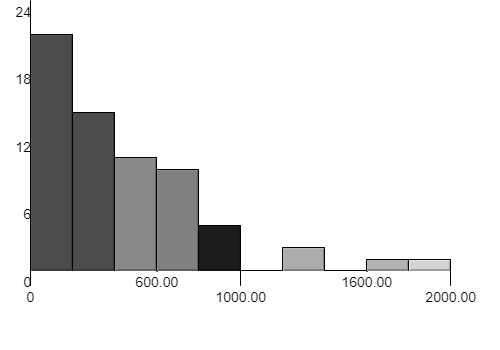
\includegraphics[scale=0.3]{img/histogram.png}

\section{Parametric Families \& Method of Moments}

\subsection{Parametric Models}

\definition{Probability Density Function}
A \textit{Probability Density Function} is a function of a \textit{Continuous Random Variable}.\\
It's value at a given point gives the probability having random variable that value.\\

\definition{Probability Mass Function}
A \textit{Probability Mass Function} is a function of a \textit{Discrete Random Variable}.\\
It's value at a given point gives the probability of the random variable having that value.\\

\definition{Parametric Family}
A \textit{Parametric Family} is a collection of distributions of the same type (\textit{e.g.} Normal, Binomial, etc.) and only differ in the value of one, or more, parameter.\\
\nb The form of the distribution is a function of these parameters.\\

\remark{Parametric Family Notation}
Let $X$ represent the parametric family and $\theta$ the variable parameter. Write
\begin{itemize}
	\item[-] $f_X(x;\theta)$ for the probability density function in the parametric family.\\
	Or, $p_x(X;\theta)$ for the probability mass function if the family is discrete.
	\item[-] $\expect(X;\theta)$ for the expectation of $X$.
	\item[-] $\prob(X\in A;\theta)$ for the probability that $X\in A$.\\
	\nb This is often written as $\prob(A;\theta)$ when the random variable is obvious.
	\item[-] $F_X(x;\theta)=\prob(X\in\{y\in\real:y\leq x\};\theta)$ for the cumulative distribution function.
\end{itemize}

\remark{Estimation of $\theta$}
When trying to estimate the value of $\theta$ for a parametric family we could use a sample set, $\hat{\theta}(x_1,\dots,x_n)$.\\
However, there is a fundamental flaw in this since the value of $\hat{\theta}(x_1,\dots,x_n)$ depends on the sample which is taken.\\
An improvement to this is to use a \textit{Population of Estimators}.\\

\remark{Population of Estimators for Estimation of $\theta$}
By choosing a population of estimators $(X_1,\dots,X_n)$ to be distributed according to the parametric model, for the true value of $\theta$, we can use $\hat{\theta}(X_1,\dots,X_n)$ to estimate $\theta$.\\
The characterisation of $\hat{\theta}(X_1,\dots,X_n)$ will show us how close the estimation of an observed sample $\hat{\theta}(x_1,\dots,x_n)$ is to $\theta^*$.\\
\nb $\theta^*$ denotes the true value of $\theta$.\\

\remark{Quantity of Interest \& Estimation of Theta}
It may be the case that our \textit{Quantity of Interest} in a problem is not $\theta$ itself, but it must be a function of $\theta$, say $\tau(\theta)$.\\
Once we have calculated an estimated value of $\hat{\theta}$ we can estimate the original \textit{Quantity of Interest} using $\hat{\tau}=\tau(\hat{\theta})$.\\

\definition{Joint Probability Density of Simple Random Sample} % Define simple random sample
For a \textit{Simple Random Sample} from a distribution $f_X(x_i;\theta)$ in a parametric family we have
$$f_{X_1,\dots,X_n}(x_1,\dots,x_n;\theta)=\prod_{i=1}^n f_X(x_i;\theta)$$

\proof{Joint Probability Density of Simple Random Sample}
Since $X_1,\dots,X_n$ are independent, their joint probability density function factorises as the product of the margin density functions. Giving % Define marginal density function
$$f_{X_1,\dots,X_n}(x_1,\dots,x_n;\theta)=f_{X_1}(x_1;\theta)f_{X_2}(x_2;\theta)\dots f_{X_n}(x_n;\theta)=\prod_{i=1}^n f_X(x_i;\theta)$$

\subsection{Method of Moments Estimation}

\remark{Motivation}
The \textit{Method of Moments Estimation} relies on the idea that if data comes from a simple random sample then the sample values are representative of population values.\\
This suggests that for $k\in\nats$ the \textit{$k^{th}$ Population Moment}$\simeq$\textit{$k^{th}$ Sample Moment}.\\

\definition{Population Moment}
Assume the population random variable $X$ comes from a parametric family with parameter $\theta$.\\
For $k\in\nats$ we define the \textit{$k^{th}$ Population Moment} as
$$\expect(X^k;\theta):=\int_{-\infty}^{\infty}x^kf(x;\theta)dx$$

\definition{Sample Moment}
For a sample with data values $\{x_1,\dots,x_n\}$ for $k\in\nats$ we define the \textit{$k^{th}$ Sample Moment} as
$$m_k=\frac{1}{n}\sum_{i=1}^nx_i^k$$
\nb This is the mean value of $x^k$ in the sample.\\

\proposition{Using Method of Moments Estimation}
Given a sample $\{x_1,\dots,x_n\}$ from a parametric family, if the family has one parameter $\theta$ we define the method of moments estimator $\hat{\theta}_{mom}$ to be the solution of
$$\expect(X;\hat{\theta}_{mom})=m_1$$.\\
If the family has two parameters $\alpha,\ \beta$ define the moments of estimators $\hat{\alpha}_{mom}$ \& $\hat{\beta}_{mom}$ to be the solutions to the simultaneous equations
\[\begin{array}{rcl}
\expect(X;\hat{\alpha}_{mom},\hat{\beta}_{mom})&=&m_1\\
\expect(X^2;\hat{\alpha}_{mom},\hat{\beta}_{mom})&=&m_2
\end{array}\]
\nb For $k$ unknown parameters compare the first $k$ population \& sample moments.\\

\example{Method of Moments, Single Parameter}
Assume $\{x_1,\dots,x_n\}$ come from a simple random sample of the distribution \textit{Exponential}($\theta$), with $\theta$ unknown.\\
Here there is one unknown parameter, so we use one equation.\\
For $\theta>0$ we have $\expect(X;\theta)=\frac{1}{\theta}$.\\
By the method of moments we have $\frac{1}{\theta}=m_1=\frac{1}{n}\sum\limits_{i=1}^nx_i$.\\
Meaning $\hat{\theta}_{mom}=\frac{1}{m_1}$.\\

\example{Method of Moments, Two Parameters}
Assume $\{x_1,\dots,x_n\}$ come from a simple random sample of the distribution $\mathcal{N}(\mu,\sigma^2)$, with $\mu,\sigma^2$ unknown.\\
We have two unknown parameters, so we need two equations.
\[\begin{array}{rcl}
\expect(X;\mu,\sigma^2)&=&m_1\\
\expect(X^2;\mu,\sigma^2)&=&var(X;\mu,\sigma^2)+\expect(X;\mu,\sigma^2)^2\\
&=&m_2\\
&=&\sigma^2+m_1^2
\end{array}\]
Thus $\mu=m_1$ \& $\sigma^2=m_2-m_1^2=\frac{1}{n}\sum\limits_{i=1}^n(x_i-\bar{x})^2\approx$ Sample variance.\\

\subsection{Assessing Fit}

\remark{Motivation}
When given a random sample $\{x_1,\dots,x_n\}$ from a population whose cumulative frequency function $F_x(x;\theta)$ and probability density function $f_X(x;\theta)$ have parametric forms, and are given an estimate $\hat{theta}$.\\
We should asses how well our model fits the data by comparing the sample with the values we might expected from $F_X(x;\hat{\theta})$.\\
If there are striking or systematic differences from what we expect, our assumed model may not be appropriate.\\

\proposition{Estimation of Cumulative Frequency}
Assuming that $\{x_1,\dots,x_n\}$ come from a simple random sample and that the model $F_X(x;\theta^*)$ is correct. Then
$$\forall\ i,y\ \prob(X_i\leq y;\theta^*)=F_X(y;\theta^*)$$
This means that $|\{X_i\leq y\}|~Bin(n,F_X(y,\theta^*))$.\\
Then $\expect(|\{X_i\leq y\}|)=nF_X(y;\theta^*)$.\\
Formally we can define a distribution to estimate $F_X(y;\theta^*)$
$$\hat{F}(y):=\frac{1}{n}|\{X_i\leq y\}|$$

\definition{Empirical Distribution Function}
The \textit{Empirical Distribution Function} is defined to be the map
$$y\mapsto\hat{F}(y)$$

\proposition{Assessing Fit}
We compare the \textit{Empirical Distribution Function} ($y\mapsto\hat{F}(y)$) to the function $y\mapsto F_X(y;\theta^*)$ to asses fit.\\
This is comparing expected values to real values.\\
Since $\theta^*$ is unknown then we use our estimate $\hat{\theta}$.\\

\definition{Probability Plot}
A \textit{Probability Plot} is a plot of the curve $y\mapsto(F_X(y;\hat{\theta}),\hat{F}(y))$.\\
If these two functions are the same then the plot will lye on the main diagonal.\\
\nb $\hat{F}(x_{(k)})=\frac{k}{n}$.\\

\definition{(Q-Q) Plots}
(Q-Q) plots share the same idea as \textit{Probability Plot}, but plot the inverse of each cumulative frequency functions (\textit{i.e.} the map $y\mapsto(F_X^{-1}(y;\hat{\theta}),\hat{F}^{-1}(y))$.\\
\nb Since $y\mapsto F_X(y;\theta)$ is continuous \& increasing, its inverse always exists.\\

\proposition{Finding $\hat{F}^{-1}(y)$}
Since $\hat{F}(x_{(k)})=\frac{k}{n}$ then $\hat{F}^{-1}(\frac{k}{n})=x_{(k)}$.\\
We can restrict the (Q-Q) plot to $k\mapsto(y_{k/n}=F_X^{-1}(\frac{k}{n};\hat{\theta}),x_{(k)})$ and then visually assess whether $x_{(k)}\simeq y_{k/n}$ for $k\in[1,n]$.\\

\proposition{Producing (Q-Q) Plots}
This technique requires an analytic or numerical method for computing values of $F_X^{-1}(x;\theta)$.
\begin{enumerate}[label=\roman*)]
	\item Compute an estimate $\hat{\theta}$ for $\theta$. (e.g. The method of moments estimate).
	\item Order the observations to obtain the order statistics $x_{(1)},\dots,x_{(n)}$.
	\item For $k=1,\dots,n$ compute $F_X^{-1}\left(\frac{k}{n+1};\hat{\theta}\right)$.\\
	\nb	These are the fitted quantile values.
	\item For $k=1,\dots,n$ plot the pairs $\left(F_X^{-1}\left(\frac{k}{n+1};\hat{\theta}\right),x_{(k)}\right)$.
	\item Add the line $y=x$ to the plot.
\end{enumerate}

\proposition{Producing Probability Plots}
This process is very similar to that for \textit{(Q-Q) Plots}.\\
This technique requires an analytic or numerical method for computing values of $F_X(x;\theta)$.
\begin{enumerate}[label=\roman*)]
	\item Compute an estimate $\hat{\theta}$ for $\theta$. (e.g. The method of moments estimate).
	\item Order the observations to obtain the order statistics $x_{(1)},\dots,x_{(n)}$.
	\item For $k=1,\dots,n$ compute $F_X\left(\frac{k}{n+1};\hat{\theta}\right)$.\\
	\nb	These are the fitted quantile values.
	\item For $k=1,\dots,n$ plot the pairs $\left(F_X\left(\frac{k}{n+1};\hat{\theta}\right),x_{(k)}\right)$.
	\item Add the line $y=x$ to the plot.
\end{enumerate}

\proposition{Interpreting Quantile Plots}
%TODO

\section{Likelihood \& Maximum Likelihood Estimation}

\definition{Likelihood Function}
Fora a given observation $x$ the \textit{Likelihood Function} is defined as
$$L(\theta;x):=\begin{cases}p(x;\theta)&\mathrm{when\ }x\mathrm{\ is\ discrete valued}\\f(x;\theta)&\mathrm{when\ }x\mathrm{\ takes\ continuous\ values}\end{cases}$$

\definition{Maximum Likelihood Estimate}
The value of $\theta$ that maximises the \textit{likelihood function} $L(\theta;x)$ is called the \textit{Maximum Likelihood Estimate} of $\theta$.\\

\remark{Motivation}
Consider trying to establish whether a given coin is fair.\\
Define $\theta:=\prob(H)$. We can gain information about $\theta$ by repeatedly tossing a coin until we get a Head.\\
Define $X$ to be the number of the toss on which we get our first head.\\
Assuming each toss is independent then $X~Geom(\theta)$ and $p(x;\theta)=(1-\theta)^{x-1}\theta$.\\
Say we perform the experiment once and get the single observation that $x=4$.\\
We get $L(\theta;x)=L(\theta;4)=p(4;\theta)=(1-\theta)^4\theta$.\\
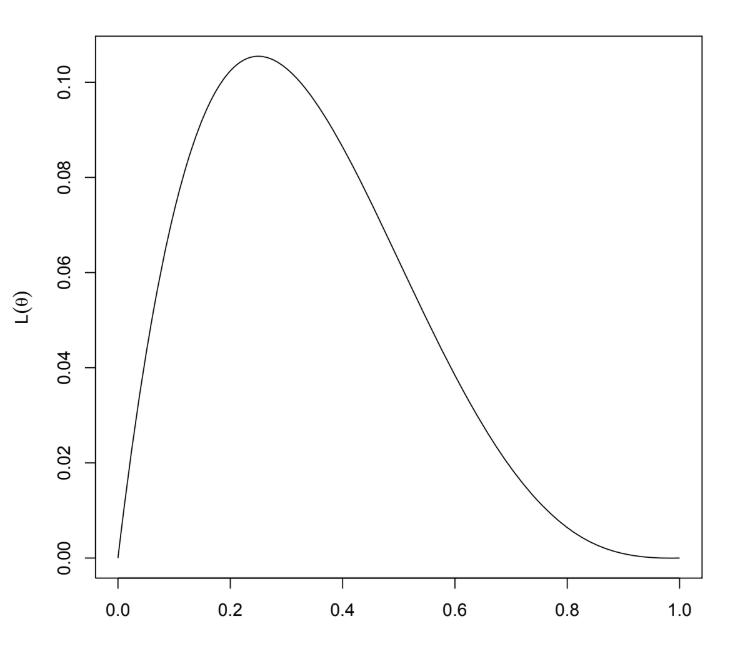
\includegraphics[scale=0.25]{img/likelihoodMotivation.png}\\
The maximum of this graph is the \textit{Maximum Likelihood Estimate} of $\theta$.\\

\example{Cont. Motivation}
We can find the turning points by setting $\frac{dL}{d\theta}=0$
\[\begin{array}{rcl}
\frac{dL}{d\theta}&=&\frac{d}{d\theta}\theta(1-\theta)^3\\
&=&(1-\theta)^3-3\theta(1-\theta)^2\\
&=&(1-\theta)^2(1-4\theta)\\
\implies\theta&=&1,\frac{1}{4}
\end{array}\]
To check which is the maximum we calculate $\frac{d^2L}{d\theta^2}$.
\[\begin{array}{rcl}
\frac{d^2L}{d\theta^2}&=&-2(1-\theta)(1-4\theta)-4(1-\theta)^2\\
\theta=\frac{1}{4}&\equiv&-2.25<0
\end{array}\]
Making $\frac{1}{4}$ is a maximum $\implies\hat{\theta}_{MLE}=\frac{1}{4}$.\\

\proposition{}
If $X_1,\dots,X_n$ is a random sample of size $n$ from a distribution with pmf $p(x;\theta)$ or pdf $f(x;\theta)$ then the $X_i$ are iid and their joint distribution factorises into teh product of marginals. Thus we can define the \textit{Likelihood Function} as
$$L(\theta;x_1,\dots,x_n):=\begin{cases}p(x_1;\theta)\dots p(x_n;\theta)& \mathrm{Discrete}\\f(x_1;\theta)\dots f(x_n;\theta)& \mathrm{Continuous}\end{cases}$$

\definition{Maximum Likelihood Estimator, Multiple Samples}
For observed values $\{x_1,\dots,x_n\}$ the maximum likelihood estimator $\hat{\theta}_{MLE}(x_1,\dots,x_n)$ is the value of $\theta$ which maximises the likelihood function $L(\theta;x_1,\dots,x_n)$.\\

\example{Multiple Samples}
Suppose we repeat the experiment from the motivation three times and get values $x_1=3,x_2=5,x_3=1$. Then
\[\begin{array}{rcl}
L(\theta;x_1,x_2,x_3)&=&p_{X_1,X_2,X_3}(x_1,x_2,x_3;\theta)\\
&=&(1-\theta)^{x_1-1}\theta(1-\theta)^{x_2-1}\theta(1-\theta)^{x_3-1}\theta\\
&=&(1-\theta)^3\theta(1-\theta)^4\theta(1-\theta)^0\theta\\
&=&(1-\theta)^7\theta^3
\end{array}\]
Maximising $L(\theta)$ we get that $\hat{\theta}_{MLE}=\frac{3}{10}$.\\

\definition{Log-Likelihood Function}
For observed values $\{x_1,\dots,x_n\}$ and associated likelihood function $L(\theta;x_1,\dots,x_n)$ the \textit{log-likelihood function} is defined as
$$\ell:=\ln L(\theta;x_1,\dots,x_n)$$
\nb Since $\ln$ is an increasing function the maximum of $L(\theta)$ \& $\ell(\theta)$ is the same.\\

\theorem{Log-Likelihood Function, Multiple Samples}
For observations from a simple random sample
$$l(\theta;x_1,\dots,x_n)=\begin{cases}\sum\limits_{i=1}^n\ln p(x_i;\theta)& \mathrm{Discrete}\\\sum\limits_{i=1}^n\ln f(x_i;\theta)& \mathrm{Continuous}\end{cases}$$

\proof{Log-Likelihood Function, Multiple Samples}
For the continuous case we have
\[\begin{array}{rcl}
\ell(\theta)&=&\ln L(\theta)\\
&=&\ln (f(x_1;\theta)\dots f(x_n;\theta))\\
&=&\ln f(x_1;\theta)+\dots+\ln f(x_n;\theta)\\
&=&\sum_i\ln f(x_i;\theta)
\end{array}\]
This is similarly shown for the discrete case.\\

\example{Log-Likelihood Function}
Let $\{x_1,\dots,x_n\}$ be the sample from $Exp(\theta)$.
\[\begin{array}{rcl}
L(\theta)&=&(\theta e^{-\theta x_1})\dots(\theta e^{-\theta x_n})\\
&=&\theta^ne^{-\theta(x_1+\dots+x_n)}\\
\implies\ell(\theta)&=&n\ln\theta-\theta\sum_ix_i
\end{array}\]

\proposition{Calculating $\hat{\theta}_{MLE}$ in Random Sample Case}
Let $f(x;\theta)$ be the pdf a continuous regular distribution.\\
Here is a technique for calculating $\hat{\theta}_{MLE}$ for a random sample.
\begin{enumerate}[label=\roman*)]
	\item Calculate $\frac{\partial}{\partial\theta}\ln f(x;\theta)$.
	\item Compute \& Simplify $\frac{d}{d\theta}\ln f(x_i;\theta)+\dots+\frac{d}{d\theta}\ln f(x_n;\theta)$.
	\item The \textit{Maximum Likelihood Estimator} is the value of $ii)=0$.
\end{enumerate}

\subsection{Maximum Likelihood Estimate of $\tau(\theta)$}

\theorem{Maximum Likelihood Estimate of $\tau(\theta)$}
Suppose our quantity of interest is a function is a continuously differentiable function $\tau(\theta)$, which is either increasing, or decreasing.\\
We can calculate the \textit{Maximum Likelihood Estimate} of $\tau(\theta)$ by plugging in $\hat{\theta}_{MLE}$
$$\widehat{\tau(\theta)}_{MLE}=\tau(\hat{\theta}_{MLE})$$

\proof{Maximum Likelihood Estimate of $\tau(\theta)$}
\textit{This is non-examinable}.\\
Under the new parametrisation we have that $\ell^{new}(\tau(\theta))=\ell^{old}(\theta)$.\\
By applying the chain rule to $\ell(\tau(\theta))$ we get
$$\frac{\partial}{\partial\theta}\ell^{old}(\theta)=\frac{\partial}{\partial\theta}\ell^{new}(\tau(\theta))=\frac{\partial}{\partial\tau(\theta)}\ell^{new}(\tau(\theta))\times\tau'(\theta)$$
Since $\tau(\theta)$ is increasing or decreasing then $\tau'(\theta)\neq0$, thus the last expression equals 0 iff $\frac{\partial}{\partial\tau(\theta)}\ell^{new}(\tau(\theta))\times\tau'(\theta)$.\\

\example{}
Let $x_1,\dots,x_n$ be observed values of a simple random variable from $Exp(\theta)$ distribution with $\theta$ unknown.\\
We found previously that $\hat{\theta}_{MLE}=\frac{1}{\bar{x}}$.\\
Consider the following functional quantities
\begin{enumerate}[label=\roman*)]
\item Suppose we are interested in the population variance.\\
Set $\tau(\theta)=Var(X;\theta)=\frac{1}{\theta^2}$. Then
$$\widehat{\tau(\theta)}=\tau(\hat{\theta})=\bar{x}^2$$
\nb This is not the same as the sample variance.
\item Suppose we are interested in the proportion of the population which have values $\geq1$.\\
Set $\tau(\theta)=\prob(X\geq1;\theta)=e^{-\theta}$. Then
$$\widehat{\tau(\theta)}=\tau(\hat{\theta})=e^{-\hat{\theta}}=exp\left(\frac{-1}{\bar{x}}\right)$$
\nb This is not the same as the sample variance of values $\geq1$.
\end{enumerate}

\subsection{Most Likelihood Estimates with Multiple Parameters}

\remark{Most Likelihood Estimates with Multiple Parameters with Regular Distributions}
\textit{Most Likelihood Estimates} can be extended to the case with multiple parameters.\\
Consider the case with two parameters $\alpha$ \& $\beta$, we can find $\hat{\alpha}_{MLE}$ \& $\hat{\beta}_{MLE}$ by solving the simultaneous solution to the two likelihood equations
$$0=\sum_{i=1}^n\frac{\partial}{\partial\alpha}\ln f(x_i;\alpha,\beta)\quad\&\quad0=\sum_{i=1}^n\frac{\partial}{\partial\beta}\ln f(x_i;\alpha,\beta)$$

\example{Multiple Parameters, Regular Density}
Consider a simple random sample from $N(\mu,\sigma^2)$, with unknown mean \& variance. (\textit{N.B.} The Normal distribution is continuous \& regular).\\
$\hat{\mu}_{MLE}$ \& $\hat{\sigma}_{MLE}$ are the simultaneous solutions to the likelihood equations.\\
Since $f(x;\mu,\sigma)=\frac{1}{\sqrt{2\pi\sigma^2}}exp(-\frac{(x-\mu)^2}{2\sigma^2})$ we have
\[\begin{array}{rrcl}
&\ln f(x;\mu,\sigma)&=&-\frac{1}{2}\ln(2\pi)-\ln(\sigma)-\frac{(x-\mu)^2}{2\sigma^2}\\
\implies&\frac{\partial}{\partial\mu}\ln f(x;\mu,\sigma^2)&=&\frac{x-\mu}{\sigma^2}\\
\mathrm{Setting}&0&=&\sum_{i=1}^n\frac{x_i-\hat{\mu}_{mle}}{\hat{\sigma}_{mle}^2}\\
&&=&\frac{1}{\hat{\sigma}_{mle}^2}\left(-n\hat{\mu}_{mle}+\sum_{i=1}^nx_i\right)\\
\implies&\hat{\mu}_{MLE}&=&\frac{1}{n}\sum_{i=1}^nx_i\\
&&=&\bar{x}
\end{array}\]
Also
\[\begin{array}{rrcl}
&\frac{\partial}{\partial\sigma}\ln f(x;\mu,\sigma^2)&=&-\frac{1}{\sigma}+\frac{x-\hat{\mu}_{mle}}{\sigma^3}\\
\mathrm{Setting}&0&=&\sum_{i=1}^b\left(-\frac{1}{\hat{\sigma}_{mle}}+\frac{x-\hat{\mu}_{mle}}{\hat{\sigma}_{mle}^3}\right)\\
\implies&\frac{n}{\hat{\sigma}_{mle}}&=&\sum_{i=1}^n\frac{(x_i-\hat{\mu}_{mle})^2}{\hat{\sigma}_{mle}^2}\\
\implies&\hat{\sigma}_{mle}^2&=&\frac{1}{n}\sum_{i=1}^n(x_i-\hat{\mu}_{mle})^2\\
&&=&var(X)
\end{array}\]

\remark{Non-Regular Density}
When the density is non-regular we cannot consider the maximum likelihood to be a turning point. Instead, the likelihood is maximised at one end-point of the interval.\\
Thus we work with $L(\theta)$ directly.\\

\example{Non-Regular Density}
Consider a simple random sample $\{x_1,\dots,x_n\}$ from the distribution $U(0,\theta)$.\\
Here $f(x;\theta)=\begin{cases}\frac{1}{\theta}&if\ 0\leq x\leq\theta\\0&otherwise\end{cases}$. Thus
$$L(\theta;x_1,\dots,x_n)=f(x_1;\theta)\dots f(x_n;\theta)=\begin{cases}\frac{1}{\theta^n}&if\theta\geq x_1,\dots,\theta\geq x_nn\\0&otherwise\end{cases}$$
Hence, the likelihood is $\frac{1}{\theta^n}$ if $\theta\geq x_{(n)}=max(x_1,\dots,x_n)$, otherwise it is 0.\\
This means that the likelihood is maximised for $\hat{\theta}_{MLE}=x_{(n)}$.\\
\nb This is easiest to see once you have plotted a graph.\\

\example{Poisson Data with Unequal Means}
Consider counting photons arriving at a detector in intervals of variable length.\\
Suppose the arrival is $\lambda$ per unit time and $X_i$ be the number of arrivals in the $i^{th}$ interval, with known time $t_i$.\\
Assume $X_i~Poisson(\lambda t_i)$ for $i\in[1,n]$ \& that the intervals don't overlap.\\
The joint probability mass function of $X_1,\dots,X_n$ is
\[\begin{array}{rrcl}
&\prob(X_1=x_1,\dots,X_n=x_n)&=&\prob(X_1=x_1)\dots\prob(X_n=x_n)\\
&&=&\frac{1}{x_1!}e^{-\lambda t_1}(\lambda t_1)^{x_1}\times\dots\times\frac{1}{x_n!}e^{-\lambda t_n}(\lambda t_n)^{x_n}\\
&&=&\dfrac{t_1^{x_1}\dots t_n^{x_n}}{x_1!\dots x_n!}e^{-\lambda(t_1+\dots+t_n)}\lambda^{x_1+\dots+x_n}\\
\implies&\ell(\lambda)&=&-\lambda(t_1+\dots+t_n)+\ln\lambda(x_1+\dots+x_n)+non-\lambda\ terms\\
\implies&\frac{\partial}{\partial\lambda}\ell(\lambda)&=&-(t_1+\dots+t_n)+\frac{1}{\lambda}(x_1+\dots+x_n)\\
\mathrm{Setting}&\frac{\partial}{\partial\lambda}\ell(\lambda)&=&0\\
\implies&\hat{\lambda}_{mle}&=&\frac{x_1+\dots+x_n}{t_1+\dots+t_n}
\end{array}\]

\section{Assessing the Performance of Estimators}

\subsection{Different Methods of Estimation}

\remark{Direct Method}
There may be a direct (non-parametric) way to estimate a population value.\\
\textit{i.e.} By analysing the sample data.\\

\example{Different Methods}
Consider estimating the population median of $U[0,\theta]$ with $\theta$ unknown.\\
The parametric method uses the function $\tau(\theta)=\frac{\theta}{2}$.\\
Considering different methods for this estimation we get
\begin{enumerate}[label=\roman*)]
	\item The \textit{Method of Moments} finds $\hat{\theta}_{mom}=2\bar{x}\implies\hat{\tau}=\bar{x}$;
	\item The \textit{Maximum Likelihood Estimates} $\hat{\theta}_{mle}=x_{(n)}\implies\hat{\tau}=\frac{x_{(n)}}{2}$;
	\item The \textit{Non-Parametric Method} gives the sample mean.
\end{enumerate}
\nb We are given 3 different values for the same quantity, for the same sample.\\

\subsection{Repeated Sampling \& Sampling Distributions}

\definition{Sampling Distributions}
Let $X_1,\dots,X_n$ be random variables.\\
The \textit{Sampling Distribution} is the distribution of the estimator $\hat{\theta}(X_1,\dots,X_n)$.\\

\remark{Good Estimator}
A \textit{Good Estimator} should be one whose distribution is concentrated close to the true value.\\

\example{Normal Distribution Sampling Distribution}
Let $X_1,\dots,X_n\sim N(\mu,\sigma^2)$.\\
From previous examples, we know $\mu_{mom}=\bar{x}\implies\hat{\mu}_{mom}\sim N\left(\mu,\frac{\sigma^2}{n}\right)$

\definition{Bias \& Mean Square Error}
Let $\hat{\theta}$ be an estimator of $\theta$.\\
We define two properties
\begin{enumerate}[label=\roman*)]
	\item $bias(\hat{\theta};\theta)=\expect(\hat{\theta}-\theta;\theta)=\expect(\hat{\theta};\theta)-\theta$.
	\item Mean Square Error, $mse(\hat{\theta},\theta)=\expect[(\hat{\theta}-\theta)^2;\theta]$.
\end{enumerate}
\nb Bias quantifies systematic error.\\

\definition{Unbiased}
We say an estimator $\hat{\theta}$ is \textit{Unbiased} if $bias(\hat{\theta};\theta)=0\ \forall\ \theta$.\\

\proposition{Mean Square Error Identity}
$$mse(\hat{\theta};\theta)=Var(\hat{\theta};\theta)+bias(\hat{\theta};\theta)^2$$

\proof{Mean Square Error Identity}
\[\begin{array}{rcl}
mse(\hat{\theta})&=&\expect[(\hat{\theta}-\theta)^2]\\
&=&\expect[(\hat{\theta}-\expect(\hat{\theta})+\expect(\hat{\theta})-\theta))^2;\theta]\\
&=&\expect[(\hat{\theta}-\expect(\hat{\theta}))^2]+\expect[(\expect(\hat{\theta})-\theta)^2]+2\expect[(\hat{\theta}-\expect(\hat{\theta}))(\expect(\hat{\theta})-\theta)]\\
&=&Var(\hat{\theta})+(\expect(\hat{\theta})-\theta)^2+2(\expect(\hat{\theta})-\theta)\expect(\hat{\theta}-\expect(\hat{\theta}))\\
&=&Var(\hat{\theta})+(\expect(\hat{\theta})-\theta)^2+2(\expect(\hat{\theta})-\theta))\times0\\
&=&Var(\hat{\theta})+bias(\hat{\theta})^2
\end{array}\]

\example{}
From the previous example we have $\hat{\mu}_{mom}\sim N\left(\mu,\frac{\sigma^2}{n}\right)$.\\
We deduce
$$bias(\hat{\mu}_{mom};\mu,\sigma^2)=\expect(\hat{\mu}_{mom};\mu,\sigma^2)-\mu=\mu-\mu=0$$
Thus
$$mse(\hat{mu}_{mom};\mu, \sigma^2)=Var(\hat{mu}_{mom};\mu, \sigma^2)+bias(\hat{mu}_{mom};\mu, \sigma^2)^2=\frac{\sigma^2}{n}+0^2=\frac{\sigma^2}{n}$$

\subsection{Approximating Sampling Distributions by Simulation}

\remark{}
A more general, but empirical, approach for \textit{Approximating a Sampling Distributions} is to use a computer to perform \textit{Simulations}.\\

\definition{Simulation}
A \textit{Simulation} is the process of artificially generating a data set of independent observations from a given probability distribution.\\

\proposition{R Pseudocode}
The following R pseudocode can be used to generate $B$ data sets of size $n$ from a distribution $f$ and then approximating the sampling distribution
\begin{enumerate}
	\item Generate $nB$ values from $f$ \& group them into $B$ groups of size $n$.
	\item Calculate the estimates for each sample.
	\item Analyse the results (numerically or graphically).
\end{enumerate}
\nb When analysing we can ask questions like \textit{``What is the probability that $\hat{\theta}\geq2$ when $\theta=1$?"}.\\

\example{Graphical Summaries of Performance-Histograms}
Consider again the problem of estimating the population median for the distribution $U[0,\theta]$.\\
We can construct histograms for this as follows
\begin{enumerate}
	\item Simulate 1000 samples of size 10 from $U[0,1]$.
	\item For each sample compute the sample median, the method of moments estimate $\bar{x}$ and the maximum likelihood estimate $max\{x_1,\dots,x_{10}\}/2$
	\item Plot the histograms for the estimate for each sample using each method
\end{enumerate}
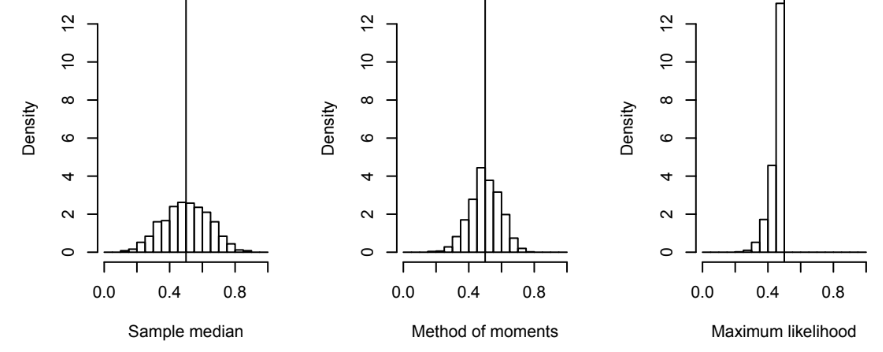
\includegraphics[scale=0.5]{img/approximateSimulation.png}

\proposition{Numerical Summaries of Performance}
We can sometimes derive explicit analytic expressions for the bias and mean-square-error of an estimator, for any value of $\theta$.\\
Say we want to estimate $\tau(\theta)$ and that we can simulate $f(\cdot;\theta)$.\\
This can be done as follows
\begin{enumerate}
	\item Generate $B$ data sets of size $n$, made of independent variables st $X_i\sim f(\cdot;\theta)$;
	\item Produce $B$ estimates of $\hat{\tau}_i=\tau(\hat{\theta}_i)$.
	\item Calculate sample mean $\bar{\tau}=\sum\limits_{i=1}^B\dfrac{\hat{\tau}_i}{B}$ \& sample variance $s=\sum\limits_{i=1}^B\dfrac{(\hat{\tau}_i-\bar{\tau})^2}{B-1}$.
	\item Compute the average error, $\bar{\tau}-\tau(\theta)$.
	\item Estimate the mean-square-error
	$$average\ squared-error=\dfrac{\sum_{i=1}^B(\hat{\tau}_i-\tau)^2}{B}$$
	$$average\ squared-error\simeq s+(average\ error)^2$$
\end{enumerate}

\subsection{Approximation Methods from the Central Limit Theorem}

\theorem{Central Limit Theorem}
Let $X_1,\dots,X_n$ be a random sample from a population with mean $\mu=\expect(X)$ \& variance $\sigma62=Var(X)$.\\
Let $\bar{X}_n=\frac{1}{n}(X_1+\dots+X_n)$ be the sample mean.\\
For large $n$, whatever the distribution of $X$
$$\prob\left(\frac{\bar{X}_n-\mu}{\sigma/\sqrt{n}}\leq x\right)\simeq\prob(N(0,1)\leq x)=\Phi(x)$$

\example{Central Limit Theorem}
Let $X_1,\dots,X_{10}$ be a random sample from $Exp(2)$.\\
Then $\mu=frac{1}{2}$ \& $\sigma^2=\frac{1}{4}$.\\
By the \textit{Central Limit Theorem}
$$\frac{\bar{X}_{10}-\mu}{\sigma/\sqrt{n}}=\frac{\frac{1}{10}(X_1+\dots+X_{10})-\frac{1}{2}}{1/(2\sqrt{10})}\simeq N(0,1)$$
If we want to approximate $\prob(X_1+\dots+X_{10}\leq5.2;\lambda=2)$ then
\[\begin{array}{rcl}
\prob(X_1+\dots+X_{10}\leq5.2;\lambda=2)&=&\prob(\bar{X}_{10}\leq\frac{5.2}{10};\lambda=2)\\
&=&\prob\left(\dfrac{\bar{X}_{10}-\frac{1}{2}}{\sqrt{1/(4\times10)}}\leq\dfrac{\frac{5.2}{10}-\frac{1}{2}}{\sqrt{1/(4\times10)}};\lambda=2\right)\\
&\simeq&\prob\left(N(0,1)\leq\dfrac{\frac{5.2}{10}-\frac{1}{2}}{\sqrt{1/(4\times10)}}\right)\\
&=&0.5503
\end{array}\]

\definition{Continuity Correction}
Let $X$ be a random variable of discrete integer values.\\
Let $T=X_1+\dots+X_n$ where $X_i$ are distributed identically \& independently to $X$.\\
Since $T$ takes integer values \textit{Continuity Correction} is used to include values that would round to target
\[\begin{array}{rcl}
\prob(T=x)&\simeq&\prob\left(x-\frac{1}{2}\leq N(n\mu,n\sigma^2)\leq x+\frac{1}{2}\right)\\
\prob(T\leq x)&\simeq&\prob\left(N(n\mu,n\sigma^2)\leq x+\frac{1}{2}\right)
\end{array}\]
\nb The \textit{Central Limit Theorem} states that $\prob(T\leq x)\simeq\prob(N(n\mu,n\sigma^2)\leq x)$ but \textit{Continuity Correction} improves the accuracy of our calculations.\\

\example{Continuity Correction}
Let $X_1,\dots,X_{10}$ be IID $Bernoulli(\frac{1}{4})$.\\
Then $\mu=\frac{1}{4}$ \& $\sigma^2=\frac{1}{4}(1-\frac{1}{4})=\frac{3}{16}$.\\
Consider $T=X_1+\dots+X_{10}$.\\
The \textit{Central Limit Theorem} suggests $T\simeq N=(n\mu,n\sigma^2)=N\left(\frac{10}{4},\frac{30}{16}\right)$.\\
Consider approximating $\prob(T\leq2)$.\\
We have that the real value is $0.5256$.\\
Using the \textit{Central Limit Theorem} we have
\[\begin{array}{rcl}
\prob(T\leq 2)&\simeq&\prob\left(N(\frac{10}{4},\frac{30}{16}\leq2\right)\\
&=&\prob\left(\dfrac{N(\frac{10}{4},\frac{30}{16})-\frac{10}{4}}{\sqrt{30/16}}\leq\dfrac{2-\frac{10}{4}}{\sqrt{30/16}}\right)\\
&=&\prob(N(0,1)\leq-0.3651)\\
&=&0.3575
\end{array}\]
Using \textit{Continuity Correction} we have
\[\begin{array}{rcl}
\prob(T\leq2)&\simeq&\prob(N(\frac{10}{4},\frac{30}{16})\leq2.5)\\
&=&\prob\left(\dfrac{N(\frac{10}{4},\frac{30}{16})-\frac{10}{4}}{\sqrt{30/16}}\leq\dfrac{2.5-\frac{10}{4}}{\sqrt{30/16}}\right)\\
&=&\prob(N(0,1)\leq0)\\
&=&0.5
\end{array}\]
Here we can see that \textit{Continuity Correction} produces a better estimation of the true value.\\

\section{Sampling Distributions Related to the Normal Distribution}

\subsection{Moment Generating Functions}

\definition{Moment Generating Function}
Let $X$ be a random variable.\\
We define the \textit{Moment Generating Function} of $X$ as
$$\mathcal{C}_X(t):=\expect(e^{tX})=\begin{cases}\int e^{tx}f_X(x)dx&\mathrm{Continuous}\\\sum_xe^{tx}\prob(X=x)&\mathrm{Discrete}\end{cases}$$

\proposition{Uniqueness of Moment Generating Function}
The \textit{Moment Generating Function} is unique for all distributions.\\
This means it can be used to show that two distributions are equivalent.\\

\proposition{Common Moment Generating Functions}
\[\begin{array}{lcll}
X\sim N(\mu,\sigma^2)&\Leftrightarrow&\mathcal{M}_X(t)=e^{\mu t+\frac{1}{2}(\sigma^2t^2)}&t\in\real\\
X\sim Exp(\theta)&\Leftrightarrow&\mathcal{M}_X(t)=\dfrac{\theta}{\theta-t}&t<\theta\\
X\sim Gamma(\alpha,\beta)&\Leftrightarrow&\mathcal{M}_X(t)=\dfrac{\beta^\alpha}{(\beta-t)^\alpha}&t<\beta
\end{array}\]

\theorem{Linear Expressions \& Moment Generating Functions}
Let $X$ \& $Y$ be random variables with $Y=aX+b$ for $a,b\in\real$. Then
$$\mathcal{M}_Y(t)=\expect(e^{tY}=\expect(e^{taX+tb})=e^{tb}\mathcal{M}_X(ta)$$

\definition{Joint Moment Generating Function}
Let $X$ \& $Y$ be random variables. Then
$$\mathcal{M}_{X,Y}(s,t):=\expect(e^{sX+tY})$$

\theorem{Marginal Moment Generating Functions}
Let $X$ \& $Y$ be random variables. Then
\[\begin{array}{rclcl}
\mathcal{M}_X(s)&=&\expect(e^{sX})&=&\mathcal{M}_{X,Y}(s,0)\\
\mathcal{M}_Y(t)&=&\expect(e^{tX})&=&\mathcal{M}_{X,Y}(0,t)
\end{array}\]

\theorem{Independent Variables \& Moment Generating Function}
Let $X$ \& $Y$ be random variables.\\
$X$ \& $Y$ are independent iff
$$\mathcal{M}_{X,Y}(s,t)=\mathcal{M}_X(s)\mathcal{M}_Y(t)=\mathcal{M}_{X,Y}(s,0)\mathcal{M}_{X,Y}(0,t)$$

\remark{Sum of Independent Variables \& Moment Generating Function}
Let $X_1,\dots,X_n$ be iid \& define $Y=X_1+\dots+X_n$. Then
$$\mathcal{M}_Y(t)=\mathcal{M}_{X_1}(t)\mathcal{M}_{X_2}(t)\dots\mathcal{M}_{X_n}(t)$$

\subsection{Transforming, Adding \& Sampling Normals}

\theorem{Linear Combinations on Normal Distribution}
Let $X\sim N(\mu,\sigma^2)$. Then
\[\begin{array}{rcl}
aX+b&\sim&N(a\mu+b,a^2\sigma^2)\\
\dfrac{X-\mu}{\sigma}&\sim&N(0,1)
\end{array}\]
\nb The second result is an implementation of the first where $a=\frac{1}{\sigma}$ \& $b=\frac{-\mu}{\sigma}$.\\

\proof{Linear Combinations on Normal Distribution}
We know that $\mathcal{M}_X(t)=e^{\mu t+\frac{1}{2}(\sigma^2t^2)}$. Then\\
\[\begin{array}{rcl}
\mathcal{M}_{aX+b}(t)&=&e^{bt}\mathcal{M}_X(at)\\
&=&e^{bt}e^{\mu at+\frac{1}{2}(\sigma^2a^2t^2)}\\
&=&e^{(\mu a+b)t+\frac{1}{2}(\sigma^2a^2t^2)}\\
\end{array}\]
This is the moment generating function for $N(a\mu+b,a^2\sigma^2)$.\\
For the second part we notice that
$$\sqrt{n}\left(\frac{\bar{X}-\mu}{\sigma}\right)=\frac{\sqrt{n}}{\sigma}\bar{X}-\frac{\sqrt{n}}{\sigma}\mu\equiv a\bar{X}+b$$
We apply $a\bar{X}+b\sim N(a\mu-b,a^2\frac{\sigma^2}{n})$ we get
$$\sqrt{n}\left(\frac{\bar{X}-\mu}{\sigma}\right)\sim N\left(\frac{\sqrt{n}}{\sigma}\mu-\frac{\sqrt{n}}{\sigma}\mu,\frac{n}{\sigma^2}\frac{\sigma^2}{n^2}\right)=N(0,1)$$

\theorem{Adding Normal Distributions}
Let $X_1,\dots,X_n$ be iid st $X_i\sim N(\mu_i,\sigma_i^2)$.\\
Then for any linear combination we have
$$\sum_ia_iX_i\sim N\left(\sum_ia_i\mu_i,\sum_ia_i^2\sigma^2_i\right)$$

\proof{Adding Normal Distributions}
\[\begin{array}{rcl}
\mathcal{M}_{\sum a_iX_i}(t)&=&\prod_{i=1}^n\mathcal{M}_{a_iX_i}(t)\\
&=&\prod_{i=1}^n\mathcal{M}_{X_i}(a_it)\\
&=&\prod_{i=1}^n\mathrm{exp}(\mu_ia_it+\frac{1}{2}\sigma_i^2a_i^2t^2)\\
&=&\mathrm{exp}\left(\left(\sum_{i=1}^n\mu_ia_i\right)+\frac{t^2}{2}\left(\sum_{i=1}^n\sigma_i^2a_i^2\right)\right)
\end{array}\]
This is the moment generating function of $N(\sum_ia_i\mu_i,\sum_ia_i^2\sigma_i^2)$.\\

\theorem{Independence of $\bar{X}$ and $\sum\limits_{j=1}^n(X_j-\bar{X})^2$}
If $X_1,\dots,X_n$ are a random sample of size $n$ from $N(\mu,\sigma^2)$ distribution then
\begin{center}
$\bar{X}$ and $\sum\limits_{j=1}^n(X_j-\bar{X})^2$ are independent.
\end{center}
\nb The proof of this is non-examinable.

\subsection{$\chi^2$ Distribution}

\definition{$\chi^2$ Distribution}
We say that a random variable $W$ has the $\chi^2$ distribution with $r$ degrees of freedom.\\
We write $W\sim\chi^2_r$ if $W$ has moment generating function
$$\mathcal{M}_W(t)=(1-2t)^{-r/2}\quad t<\frac{1}{2}$$

\remark{Symmetry of $\chi^2$}
$\chi^2$ cannot be symmetric around zero as it only takes positive values.\\

\remark{$\chi^2$ \& Gamma Distribution}
By comparison of moment generating functions we have that
$$\chi^2_r\equiv\Gamma\left(\frac{r}{2},\frac{1}{2}\right)$$

\proposition{Expectation \& Variance of $\chi^2$ Distribution}
If $W\sim\chi^2_r$ then
$$\expect(W)=\frac{r/2}{1/2}=r\quad Var(W)=\frac{r/2}{(1/2)^2}=2r$$

\remark{$\chi^2$ is Squared Normal}
If $Z\sim N(0,1)$ then $Y=Z^2\sim\chi^2_1$.\\

\proof{$\chi^2$ is Squared Normal}
Below we show that when $t<\frac{1}{2}$ then the squared normal distribution has the same moment generating function as $\chi^2_1$.
\[\begin{array}{rcll}
\mathcal{M}_Y&=&\expect(e^{tY})=\expect(e^{tZ^2})\\
&=&\int_{-\infty}^\infty e^{tz^2}\prob(Z=z)dz\\
&=&\int_{-\infty}^\infty e^{tz^2}\frac{1}{\sqrt{2\pi}}e^{\frac{1}{2}z^2}dz\\
&=&\frac{1}{\sqrt{2\pi}}\int_{-\infty}^\infty exp(-\frac{1}{2}(z^2-2tz^2))dz\\
&=&\frac{1}{\sqrt{2\pi}}\int_{-\infty}^\infty exp(-\frac{1}{2}z^2(1-2t))dz\\
&=&\frac{1}{\sqrt{2\pi}}\int_{-\infty}^\infty exp(-\frac{1}{2}z^2/\frac{1}{1-2t})dz\\
&=&\frac{1}{\sqrt{2\pi}}\times\sqrt{2\pi\sigma^2}&\mathrm{Where}\ \sigma^2=\frac{1}{1-2t}\\
&=&\sigma=\frac{1}{\sqrt{1-2t}}
\end{array}\]

\theorem{Sum of $\chi^2$ Distributions}
The following hold $\forall\ r,s$
\begin{enumerate}[label=\roman*)]
	\item If $U\sim\chi^2_r$ \&  $U\sim\chi^2_s$ are independent, then  $U+V\sim\chi^2_{r+s}$.
	\item If $Z_i^2\sim N(0,1)$ are independent then $\sum_i Z_i^2\sim\chi^2_n$.
\end{enumerate}

\proof{Sum of $\chi^2$ Distributions}
Consider the moment generating function of $U+V$
\[\begin{array}{rcl}
\mathcal{M}_{U+V}(t)&=&\mathcal{M}_U(t)+\mathcal{M}_V(t)\\
&=&\frac{1}{(1-2t)^{r/2}}\times\frac{1}{(1-2t)^{s/2}}\\
&=&(1-2t)^{-\frac{1}{2}(r+s)}
\end{array}\]
So $t\in[0,\frac{1}{2}]$ and we recognise the moment generating function of $chi^s_{r+s}$

\subsection{Normal Sampling Distribution}

\theorem{}
Let $X_1,\dots,X_n$ be a random sample of size $n$ from $N(\mu,\sigma^2)$. Then
\begin{enumerate}[label=\roman*)]
	\item $\sum_i\frac{1}{\sigma^2}(X_j-\mu)^2\sim\chi_n^2$; and
	\item $\sum_i\frac{1}{\sigma^2}(X_j-\bar{X})^2\sim\chi_{n-1}^2$.
\end{enumerate}

\proof{Theorem 5.8}
\begin{enumerate}[label=\roman*)]
	\item Writing $Y_i=\frac{1}{\sigma}(X_i-\mu)$ we have $Y_i\sim N(0,1)$.\\
	Further $Y_i$ are independent of $\sum_iY_i^2\sim\chi_n^2$.\\
	But $\sum_i\frac{1}{\sigma^2}(X_i-\mu)^2=\sum_iY_i^2$.
	\item We have
	$$\sum_{i=1}^nY_i^2=\sum_{i=1}^n(Y_i-\bar{Y}+\bar{Y})^2=\sum_{i=1}^n\left[(Y_i-\bar{Y})^2+\bar{Y}^2+2\bar{Y}(Y_i-\bar{Y})\right]$$
	Note that $\bar{Y}\sum_{i=1}^n(Y_i-\bar{Y})=0$.\\
	Let $W_1=\sum_{i=1}^n(Y_i-\bar{Y})^2$ and $W_2=nY^2$.\\
	Then $\sum_{i=1}^nY_i^2=W_1+W_2=W_3$.\\
	We have $W_1$ \& $W_2$ are independent therefore
	$$\mathcal{M}_{W_3}(t)=\mathcal{M}_{W_1}(t)\mathcal{M}_{W_2}(t)\implies\mathcal{M}_{W_1}(t)=\frac{\mathcal{M}_{W_3}(t)}{\mathcal{M}_{W_2}(t)}$$
	Notice that $\sqrt{n}\bar{Y}=\sqrt{n}\left(\dfrac{\bar{X}-\mu}{\sigma}\right)\sim N(0,1)$.\\
	Thus $W_1\sim\chi^2_1$.\\
	Therefore $\mathcal{M}_{W_3}(t)=\dfrac{(1-2t)^{-n/2}}{(1-2t)^{-1/2}}=(1-2t)^{\frac{1}{2}(n-1)}$.
\end{enumerate}

\subsection{t-Distribution}

\definition{t-Distribution}
Let $U$ \& $V$ be independent random variables with $U\sim N(0,1)$ \& $V\sim\chi_r^2$.\\
Define $W=\dfrac{U}{\sqrt{V/r}}$. We say
$$W\sim t_r$$

\theorem{Variance \& Expectation of t-Distribution}
Let $W\sim t_r$ then
$$\expect(W)=0\quad Var(W)=\dfrac{r}{r-2}$$

\proposition{Properties of t-Distribution}
Let $W\sim t_r$. Then
\begin{enumerate}[label=\roman*)]
	\item $W$ is symmetric about 0;
	\item $W$ is similar to $N(0,1)$ but with heavier tails; and,
	\item As $r\to\infty$ we have $W\to N(0,1)$.
\end{enumerate}

\theorem{}
Let $X_1,\dots,X_n$ be a random sample from $N(\mu,\sigma^2)$.\\
Define $\bar{X}=\frac{1}{n}\sum_iX_i$ \& $S^2=\frac{1}{n-1}\sum_i(X_i-\bar{X})^2$.\\
We can define
\begin{enumerate}[label=\roman*)]
	\item $U:=\frac{\sqrt{n}}{\sigma}(\bar{X}-\mu)\sim N(0,1)$;
	\item $V:=\frac{1}{\sigma^2}\sum_i(X_i\bar{X})^2$.
\end{enumerate}
Then
\begin{enumerate}
	\item $U$ \& $V$ are independent; and
	\item $\frac{\sqrt{n}}{S}(\bar{X}-\mu)\sim t_{n-1}$.
\end{enumerate}
This result allows us to know how far apart we expect $\mu$ \& $\bar{X}$ to be, even when $\sigma^2$ is unknown.\\

\proof{Theorem 5.10}
We have $\dfrac{S^2}{\sigma^2}=\dfrac{V}{n-1}\sim\dfrac{\chi_{n-1}^2}{n-1}$.\\
$U$ \& $V$ are independent by \textbf{Theorem 5.6}.\\
The result is proved by
$$\frac{\sqrt{n}}{S}(\bar{X}-\mu)=\left(\frac{\sqrt{n}}{S}(\bar{X}-\mu)\right)\frac{1}{\sqrt{S^2/\sigma^2}}=U\times\frac{V}{n-1}\sim \frac{N(0,1)}{\sqrt{\chi_{n-1}^2/(n-1)}}$$
These terms are independent as required.

\subsection{Percentage Points of Distributions}

\definition{Percentage Points}
For a given $\alpha\in[0,1]$ we define the \textit{Percentage Point} $x_\alpha$ to be the value where
$$\prob(X\geq x_\alpha)=\alpha$$.\\
\nb Usually we use values of the magnitude of$\alpha=0.1,0.05,0.025,\dots$.\\

\proposition{Percentage Points of Particular Distributions}
\begin{tabular}{|l|c|c|}
\hline
RV&Notation&Symmetric around 0\\
\hline
$Z\sim N(0,1)$&$\prob(Z\geq z_\alpha)=\alpha$&Yes\\
$T\sim T_r$&$\prob(Z\geq t_{r;\alpha})=\alpha$&Yes\\
$W\sim\chi_r^2$&$\prob(W\geq \chi^2_{r;\alpha})=\alpha$&No\\
\hline
\end{tabular}
\\

\remark{Inversion of Percentage Point}
From these distributions we can deduce that
\[\begin{array}{rcl}
(1-\alpha)&=&\prob(-z_{\alpha/2}\leq Z\leq z_{\alpha/2})\\
(1-\alpha)&=&\prob(-t_{r;\alpha/2}\leq T\leq t_{r;\alpha/2})\\
(1-\alpha)&=&\prob(\chi^2_{r;1-\alpha/2}\leq W\leq\chi^2_{r;\alpha/2})
\end{array}\]

\theorem{}
Let $X_1,\dots,X_n$ be a random sample from $Exp(\theta)$. Then
\begin{enumerate}[label=\roman*)]
	\item $\sum_{i=1}^n X_i\sim\Gamma(n,\theta)$;
	\item $\bar{X}=\frac{1}{n}\sum_{i=1}^nX_i\sim\Gamma(n,n\theta)$; and,
	\item $2\theta\sum_{i=1}^nX_i\sim\Gamma(n,\frac{1}{2})=\chi^2_{2n}$.
\end{enumerate}

\section{Confidence Interval}

\definition{Confidence Interval}
Let $X_1,\dots,X_n$ be iid random variables with pmf $f_{X_1,\dots,X_n}(\cdot,\theta)$ for some $\theta$.\\
Choose $\alpha\in(0,1)$.\\
A $100(1-\alpha)\%$ \textit{Confidence Interval} for $\theta$ is a random interval of the form $(C_L,C_U)$ st
$$\prob(C_L\leq\theta^*\leq C_U;\theta)\geq1-\alpha$$
\nb $\theta^*$ is the true value of $\theta$.\\

\definition{Length of a Confidence Interval}
For a \textit{Confidence Interval} $(C_L,C_U)$ the length is defined as the range of these value
$$|C_L-C_U|$$

\proposition{Procedure for Finding Confidence Interval}
This technique depends on some statistics $f(\pmb{X})=f(X_1,\dots,X_n)$, which is generally given.
\begin{enumerate}[label=\roman*)]
	\item Treat $\theta$ as unknown;
	\item Use facts about the distribution to find an interval depending on $\theta$ st
	$$\prob(g_1(\theta^*)\leq f(\pmb{X})\leq g_2(\theta^*);\theta)=1-\alpha$$
	\item Invert the interval so that it is an inequality about $\theta$
	$$\prob(C_L(f(\pmb{X}))\leq\theta^*\leq c_U(f(\pmb{X}));\theta)=1-\alpha$$
\end{enumerate}

\example{Confidence Interval for $\mu$ in $N(\mu,\sigma^2_0)$}
Consider a sample $X_1,\dots,X_n$ from $N(\mu,\sigma_0^2)$.\\
We know $\bar{X}\sim N(\mu,\frac{1}{n}\sigma^2)$ \& $\dfrac{\bar{X}-\mu}{\sigma_0/\sqrt{n}}\sim N(0,1)$.\\
We shall calculate a confidence interval for the value of $\mu$ with $\alpha=0.05$.\\
We know that $z_{0.05/2}=z_{0.025}=1.96$. Then
$$\prob\left(-1,96\leq\frac{\bar{X}-\mu}{\sigma_0/\sqrt{n}}\leq1.96;\mu,\sigma_0^2\right)=0.95$$
But
\[\begin{array}{rrcl}
&\dfrac{\bar{X}-\mu}{\sigma_0/\sqrt{n}}&\leq&1.96\\
\implies&\bar{X}-\mu&\leq&1.96\frac{\sigma_0}{\sqrt{n}}\\
\implies&\bar{X}-1.96\frac{\sigma_0}{\sqrt{n}}&\leq&\mu
\end{array}\]
Similarly
\[\begin{array}{rrcl}
&\dfrac{\bar{X}-\mu}{\sigma_0/\sqrt{n}}&\geq&-1.96\\
\implies&\bar{X}-\mu&\geq&-1.96\frac{\sigma_0}{\sqrt{n}}\\
\implies&\bar{X}+1.96\frac{\sigma_0}{\sqrt{n}}&\geq&\mu
\end{array}\]
We have the event $\left\{-1.96\leq\dfrac{\bar{X}-\mu}{\sigma_0/\sqrt{n}}\right\}\equiv\left\{\bar{X}-1.96\frac{\sigma_0}{\sqrt{n}}\leq\mu\leq\bar{X}+1.96\frac{\sigma_0}{\sqrt{n}}\right\}$.\\
Hence
$$\prob\left(\bar{X}-1.96\frac{\sigma_0}{\sqrt{n}}\leq\mu\leq\bar{X}+1.96\frac{\sigma_0}{\sqrt{n}};\mu,\sigma_0^2\right)=0.95$$

\proposition{General Confidence Interval}
Consider a more general $100(1-\alpha)\%$ confidence interval for $\mu$ using a random sample of $N(\mu,\sigma_0^2)$.
$$\prob\left(-z_{\alpha/2}\leq\frac{\bar{X}-\mu}{\sigma_0/\sqrt{n}}\leq z_{\alpha/2};\mu;\sigma^2_0\right)=1-\alpha$$
Rearranging we find
$$\prob\left(\bar{X}-\frac{z_{\alpha/2}\sigma_0}{\sqrt{n}}\leq\mu\leq\bar{X}+\frac{z_{\alpha/2}\sigma_0}{\sqrt{n}}\right)=1-\alpha$$

\remark{Size of General Confidence Interval}
Consider the confidence interval identified in \textbf{Proposition 6.2}, we see that this interval
\begin{enumerate}[label=\roman*)]
	\item Decreases as sample size $n$ increases;
	\item Increases as population variance $\sigma^2_0$ increases;
	\item Increases as confidence level $100(1-\alpha)$ increases.
\end{enumerate}

\proposition{Confidence Interval for $\mu$ in $N(\mu,\sigma62)$ with unknown $\sigma^2$}
Let $X_1,\dots,X_n$ be a random sample from $N(\mu,\sigma^2)$ with $\sigma^2$ unknown.\\
By \textbf{Theorem 5.10} we have that
$$\dfrac{\bar{X}-\mu}{S/\sqrt{n}}\sim t_{n-1}$$
Let $T\sim t_{n-1}$ with $\prob(T\geq t_{n-1;\alpha/2})=\alpha/2$.\\
By symmetry $\prob(T\leq-t_{n-1;\alpha/2})=\alpha/2$.\\
Thus
$$\prob\left(-t_{n-1;\alpha/2}\leq\frac{\bar{X}-\mu}{s/\sqrt{n}}\leq t_{n-1;\alpha/2};\mu,\sigma^2\right)=1-\alpha$$
By rearranging
$$\prob\left(\bar{X}-\frac{St_{n-1;\alpha/2}}{\sqrt{n}}\leq\mu\leq\bar{X}+\frac{St_{n-1;\alpha/2}}{\sqrt{n}}\right)=1-\alpha$$
\nb The length of this interval is random, not fixed.

\subsection{Confidence Interval for $\sigma^2$ for $N(\mu,\sigma^2)$ Data with $\mu$ Unknown}

\proposition{Confidence Interval for $\sigma62$ for $N(\mu,\sigma^2)$ Data with $\mu$ Unknown}
Let $X_1,\dots,X_n$ be a random sample from $N(\mu,\sigma^2)$ with $\sigma^2$ unknown.\\
Then $$\frac{1}{\sigma^2}\sum_{j=1}^n(X_j-\bar{X})^2\sim\chi_{n-1}^2$$
Hence $\forall\ \alpha$
$$\prob\left(\chi_{n-1;1-\alpha/2}^2\leq\frac{1}{\sigma^2}\sum_{j=1}^n(X_j-\bar{X})^2\leq\chi_{n-1;\alpha/2}^2;\mu,\sigma^2\right)=1-\alpha$$
Rearranging we get
$$\prob\left(\frac{1}{\chi_{n-1;\alpha/2}^2}\sum_{j=1}^n(X_j-\bar{X})^2\leq\sigma^2\leq\frac{1}{\chi_{n-1;1-\alpha/2}^2}\sum_{j=1}^n(X_j-\bar{X})^2\right)=1-\alpha$$

\subsection{Confidence Interval for $\theta$ in $U(0,\theta)$}

\proposition{Confidence Interval for $\theta$ in $U(0,\theta)$}
Let $X_1,\dots,X_n$ be a random sample from $U(0,\theta)$.\\
We know that $\hat{\theta}_{MLE}=\mathrm{max}(X_1,\dots,X_n)$ so
\[\begin{array}{rcll}
prob(X_{(n)}\leq x;\theta)&=&\prob(X_1,\dots x,\dots,X_n\leq x;\theta)\\
&=&\prob(X_1\leq x;\theta)\dots\prob(X_n\leq x;\theta)&\mathrm{Independence}\\
&=&\prob(X\leq x;\theta)^n&\mathrm{Identically Distributed}\\
&=&\begin{cases}
\left(\frac{x}{\theta}\right)^n&\mathrm{if\ }1\leq x\leq\theta\\
0&\mathrm{if\ }x\leq0\\
1&\mathrm{if\ }x\geq\theta
\end{cases}
\end{array}\]
We deduce that $\frac{X_{(n)}}{\theta}$ does not depend on $\theta$.\\
$$\prob\left(\frac{X_{(n)}}{\theta}\leq\frac{x}{\theta}\right)=\left(\frac{x}{\theta}\right)^n$$
Set $u^{1/n}=\frac{x}{\theta}$
$$\implies\prob\left(\frac{X_{(n)}}{\theta}\leq u^{1/n}\right)=u$$
Let $u_1,u_2\in[0,1]$ with $u_1<u_2$
\[\begin{array}{rrcl}
&\prob\left(\frac{X_{(n)}}{\theta}\leq u_2^{1/n}\right)-\prob\left(\frac{X_{(n)}}{\theta}\leq u_1^{1/n}\right)&=&u_2-u_1\\
\equiv&\prob\left(u_1^{1/n}\leq\frac{X_{(n)}}{\theta}\leq u_2^{1/n}\right)=u_2-u_1
\end{array}\]
Choosing $u_2=1-\alpha/2$ \& $u_1=\alpha/2$ we get
$$\prob\left(\frac{X_{(n)}}{u_2^{1/n}}\leq\theta\leq\frac{X_{(n)}}{u_1^{1/n}}\right)=1-\alpha$$

\remark{The rest of chapter 6 is non-examinable}

\section{Hypothesis Testing}

\definition{Hypothesis Test}
A \textit{Hypothesis Test} is a procedure for evaluating whether sample data is consistent with one of two contrasting statements about the value of the population parameters.\\

\remark{Types of Hypothesis Tests}
Suppose we want to test the value of a parameter $\theta$, with \textit{Null Hypothesis} that $\theta=\alpha$.\\
There are three hypothesis tests we can use
\begin{enumerate}[label=\roman*)]
	\item $\theta>\alpha$;
	\item $\theta<\alpha$; and,
	\item $\theta\neq\alpha$.
\end{enumerate}

\proposition{Hypothesis Testing Procedure}
A Hypothesis test can be performed by the following procedure
\begin{enumerate}[label=\roman*)]
	\item State model assumptions,
	\item State null hypothesis \& alternative hypotheses,
	\item Choose \& calculate the value of an appropriate test statistic,
	\item Compute the resulting $p$-value.
	\item Make conclusions.
\end{enumerate}

\remark{iii) Test Statistic}
We define a suitable test statistics $T(X_1,\dots,X_n)$ which has the following properties
\begin{enumerate}[label=\roman*)]
	\item Extreme values are unlikely if $H_0$ is true;
	\item Extreme values are consistent with $H_1$; and,
	\item When $H_0$ is true then the distribution of $T$ is known and its distribution function can be easily calculated.
\end{enumerate}

\remark{iv) $p$-Value}
Let $T_{obs}$ be the observed value of the test statistic.\\
We calculate the \textit{$p$-Value} depending upon the \textit{Alternative Hypothesis}
\begin{enumerate}[label=\roman*)]
	\item $H_1:\mu>\mu_0\implies$ $p$-Value$=\prob(T\geq t_{obs}|H_0$ true$)$;
	\item $H_1:\mu<\mu_0\implies$ $p$-Value$=\prob(T\leq t_{obs}|H_0$ true$)$;
	\item $H_1:\mu\neq\mu_0\implies$ $p$-Value$=\prob(|T|\geq|t_{obs}||H_0$ true$)$;
\end{enumerate}

\remark{v) Conclusion}
If the \textit{$p$-Value} is very small we believe that the null hypothesis is false.\\

\example{Hypothesis Testing for Normal Distribution with Known Variance}
Consider a medication that hsa a mean time to recurrence of an illness of $\mu_0=53.3$, with $\sigma_0=26.4$.\\
A new medication is trialled on 16 patients. For the sample $\bar{X}=65.8$.\\
Assuming the variance is the same for both medications, does the new medication have a longer mean time to recurrence?
\begin{enumerate}[label=\roman*)]
	\item \textit{Model}.\\
	We assume the recurrence time for the patients of the new medication is distributed $N(\mu,\sigma_0^2)=N(\mu,26.4^2)$.
	\item \textit{Hypothesis}.\\
	$H_0:\mu=53.5=\mu_0$ \& $H_1:\mu>53.3=\mu_0$
	\item\textit{Test Statistics}.\\
	Define $T(X_1,\dots,X_{16})=\sqrt{n}\left(\dfrac{\bar{X}-\mu_0}{\sigma_0}\right)=\sqrt{16}\left(\dfrac{\bar{X}-53.5}{26.4}\right)$.\\
	Since $\bar{X}\sim N(\mu,\frac{\sigma_0^2}{n})$ then $T(X_1,\dots,X_{16})\sim N\left(\sqrt{n}\frac{\mu-\mu_0}{\sigma_0},1\right)$.\\
	This means that if $H_0$ is true then $T\sim N(0,1)$.\\
	We calculate the observed statistic to be $t_{obs}=\sqrt{16}\left(\frac{65.8-53.3}{26.4}\right)=1.893$.
	\item\textit{p-Value}.\\
	Here $p-value=\prob(T\geq t_{obs};\mu=\mu_0,\sigma=\sigma_0)$.\\
	Since $T\sim N(0,1)$ then
	\[\begin{array}{rcl}
	p-value&=&\prob(Z\geq t_{obs};\mu=\mu_0,\sigma=\sigma_0\\
	&=&\prob(Z\geq1.893)\\
	&=&1-\prob(Z\leq1.893)\\
	&=&1-\Phi(1.893)\\
	&=&0.0292
	\end{array}\]
	\item\textit{Conclusion}
	This value is sufficiently small, so we reject $H_0$ in favour of $H_1$.\\
\end{enumerate}

\proposition{Confidence Interval for Normal Distribution with Mean \& Variance Unknown}
\begin{enumerate}[label=\roman*)]
	\item Assume $X_1,\dots,X_n\sim(\mu,\sigma^2)$ with $\mu$ \& $\sigma^2$ unknown.
	\item Define $H_0:\mu=\mu_0$ \& $H_1=\mu\neq\mu_0$ (Other $H_1$s are possible).
	\item When $H_0$ is true $T=\dfrac{\bar{X}-\mu}{S/\sqrt{n}}\sim t_{n-1}$.
	\item Since $H_1:\mu\neq\mu_0$ we want to check the event $\{|T|\geq|t_{obs}|\}$. Then
	$$p-value=\prob(|T|\geq|t_{obs}\ |H_0\ is\ true)=\prob(|t_{n-1}|\geq|t_{obs}|) $$
\end{enumerate}

\subsection{Critical Region}

\definition{Critical Region}
the \textit{Critical Region} is the set of values, at a given significance level, which if the test-statistic falls within we reject $H_0$.\\

\definition{Critical Value(s)}
\textit{Critical Value}s are values which are the threshold for $H_0$ being rejected.\\
\nb These are denoted $c^*$.\\

\example{Critical Region}
Define $H_0:\mu=\mu_0$ \& $H_1:\mu>\mu_0$.\\
Let $T:=\sqrt{n}\frac{(\bar{X}-\mu}{\sigma_0}$ \& $\alpha$ be the significance level.\\
The the critical region is
$$C:=\{x_1,\dots,x_n\}:T(x_1,\dots,x_n)\geq c^*)\equiv\{T\geq c^*\}$$
Then
$$\prob(H_0\ is\ rejected|H_0\ true)=\prob(Type\ 1\ Error)=\alpha$$
for this example this is
$$\prob(C|H_0\ is\ True)=\prob(T\geq c^*|H_0\ is\ true)=\alpha$$
Since $T\sim N(0,1)$ we have
\[\begin{array}{rcl}
\alpha&=&\prob(T\geq c^*|H_0\ is\ true)\\
&=&\prob(|\geq c^*)\\
&-&1-\prob(|\leq c^*)\\
&=&1-\Phi(c^*)\\
\implies c^*&=&\phi^{-1}(1-\alpha)
\end{array}\]
For $\alpha=0.05\implies c^*=\phi^{-1}(0.095)=1.645$.\\
Thus we reject $H_0$ if $T\geq c^*=1.645$.\\
Equivalently, we reject if $\bar{X}\geq\mu+\frac{1.645\sigma_0}{\sqrt{n}}$ by definition of $T$.\\

\remark{Confidence Intervals \& Hypothesis Testing}
Consider using a test statistic $T$ which is normally distributed to test $H_0:\mu=\mu_0$.\\
If we know $\sigma^2=\sigma_0^2$, by hypothesis testing, we reject $H_0$ if
$$z_{\alpha/2}=c^*\leq|T|==\left|\dfrac{\sqrt{n}(\bar{X}-\mu_0)}{\sigma_0}\right|$$
Rearranging we can find a confidence interval for rejecting $H_0$
$$\mu_0\not\in\left[\bar{X}-\dfrac{c^*\sigma_0}{\sqrt{n}},\bar{X}+\dfrac{c^*\sigma_0}{\sqrt{n}}\right]$$

\section{Comparison of Population Means}

\remark{Comparing two groups}
In many real life situations we collected data in order to compare two groups.\\
There are two possible relationships these two groups can have
\begin{enumerate}[label=\roman*)]
	\item \textit{Independent Samples}.\\
	Each data set is entirely independent of one another.\\
	In this case each group can be modelled by different population distributions.\\
	\textit{e.g.} - Patients in different groups given different medication.
	\item \textit{Paired Samples}\\
	Here the data consists of pairs of observations for each member of the population.\\
	\textit{e.g.} - Patients given drug $A$ \& after some time given drug $B$
\end{enumerate}

\example{Two Sample $t$-test}
Consider being given two independent samples and asked to test whether they have the same mean.\\
Let $X_1,\dots,X_n$ be a random sample of size $n$ from $N(\mu_X,\sigma^2_X)$ \& $Y_1,\dots,Y_m$ be a random sample of size $n$ from $N(\mu_Y,\sigma^2_Y)$.\\
Define $H_0: \mu_X-\mu_Y=0$ \& $H_1:\mu_X-\mu_Y\neq0$.\\
Our standard estimators are $\bar{X}$ \& $\bar{Y}$ so our analysis will be based on the value of $\bar{X}-\bar{Y}$.\\
We have $\bar{X}\sim N\left(\mu_X,\frac{\sigma_X^2}{n}\right)$ \& $\bar{Y}\sim N\left(\mu_Y,\frac{\sigma_Y^2}{m}\right)$ so $\bar{X}-\bar{Y}\sim N\left(\mu_X-\mu_Y,\frac{\sigma_X^2}{n}+\frac{\sigma_Y^2}{n}\right)$.\\
Let $U=\dfrac{(\bar{X}-\bar{Y})-(\mu_X-\mu_Y)}{\sqrt{(\sigma_X^2/n)+(\sigma_Y^2/n)}}\sim N(0,1)$.\\
If $H_0$ is true then $U=\dfrac{\bar{X}-\bar{Y}}{\sqrt{(\sigma_X^2/n)+(\sigma_Y^2/n)}}\sim N(0,1)$.\\
If we know the variance we can compute the $p$-value \& test the hypotheses.\\
\nb Generally we have to estimate $\sigma_X^2$ \& $\sigma_Y^2$ with the sample variance.\\

\remark{Pooled Estimate, $S_p^2$}
If can assume that two samples ($X$ \& $Y$), have the same variance we can combine the estimators of their variance into a single pooled estimate $S_p^2$.
$$S_P^2=\dfrac{(n-1)S_X^2+(m-1)S_Y^2}{(n-1)+(n-1)}=\dfrac{\sum_{i=1}^n(X_i-\bar{X})^2+\sum_{i=1}^m(Y_i-\bar{Y})^2}{n+m-2}$$
Then the test statistic is $T=\dfrac{(\bar{X}-\bar{Y})}{S_P\sqrt{(1/n)+(1/m)}}\sim T_{m+n-2}$.\\
From \textbf{Theorem 5.8} $\frac{\sum_{i=1}^n(X_i-\bar{X})^2}{\sigma_X^2}\sim\chi_{n-1}^2$ \& $\frac{\sum_{i=1}^m(Y_i-\bar{Y})^2}{\sigma_Y^2}\sim\chi_{n-1}^2$.\\
Due to the independence of the samples the sum of these two result of a $\chi^2_{m+n-2}$ distribution.\\
Thus
$$\dfrac{S_p^2}{\sigma^2}=\dfrac{\sum_{i=1}^n(X_i-\bar{X})^2+\sum_{i=1}^m(Y_i-\bar{Y})^2}{\sigma^2(n+m-2}\sim\chi^2_{n+m-2)}$$
\nb From \textbf{Definition 5.4} we deduce that $T\sim t_{n+m-2}$.\\

\section{Linear Regression}

\remark{Motivation}
Here we consider a one-dimensional data set $x$ \& a linear dependent $Y=ax+b$ with $a,b\in\real$.\\

\definition{Predictor \& Response Variable}
Consider a date set $x$ \& linear dependent $Y=ax+b$.\\
Here $x$ is called the \textit{Predictor Variable} \& $Y$ is the \textit{Response Variable}.\\

\remark{Random Effects}
We need to take account of random variables in the relationship between the \textit{Predictor Variable} \& \textit{Response Variable}.\\
\textit{i.e} - If we took multiple samples of $x$ we would get different values of $Y$.\\

\definition{Linear Regression Model}
The simple \textit{Linear Regression Model} says
$$\expect(Y|x)=a+bx\ \mathrm{for}\ a,b\in\real$$
\nb - If $b=0$ then $x$ \& $Y$ are independent.\\

\proposition{Model Assumptions}
Let $\{x_1,\dots,x_n\{$ be observed values of predictor variable $x$.\\
Let $y_i$ b the response variable to $x_i$ with $Y_i=a+bx_i+e_i$ where $e_i$ is a random variable \& $a,b\in\real$ are unknown.\\
The assumptions we make are
\begin{enumerate}
	\item $\expect(e_i)=0$;
	\item $Var(e_i)=\sigma^2$ which is unknown; and,
	\item $Cov(e_i,e_j)=0$ for $i\neq j$ (\textit{i.e} Errors are uncorrelated).
\end{enumerate}

\definition{Summary Statistics}
In order to simplify notation we introduce \textit{Summary Statistics} of a data sample
\begin{itemize}
	\item[-] $\bar{x}=\frac{1}{n}\sum_{i=1}^nx_i$ \& $\bar{y}=\frac{1}{n}\sum_{i=1}^ny_i$;
	\item[-] $ss_{xx}=\sum_{i=1}^n(x_i-\bar{x})^2=\sum_{i=1}^n\left(x_i^2\right)-n\bar{x}^2$ \& $ss_{yy}=\sum_{i=1}^n(y_i-\bar{y})^2=\sum_{i=1}^n\left(y_i^2\right)-n\bar{y}^2$;
	\item[-] $ss_{xy}=\sum_{i=1}^n(x_i-\bar{x})(y_i-\bar{y})=\sum_{i=1}^n\left(x_iy_i\right)-n\bar{x}\bar{y}$.
\end{itemize}

\subsection{Least Squares Estimates}

\definition{Least Squares Estimates}
The \textit{Least Squares Estimate} is the parameter values for
$$\mathrm{argmin}_{a,b}\sum_{i=1}^n(y_i-(a+bx_i))^2$$
\nb - These values are denoted as $\hat{a}$ \& $\hat{b}$.\\

\theorem{Finding $\hat{a}$ \& $\hat{b}$}
For the simple linear regression model, the least squares estimates $\hat{a}$ \& $\hat{b}$ are given by
\begin{itemize}
	\item $\hat{b}=\frac{ss_{xy}}{ss_{xx}}$; and
	\item $\hat{a}=\bar{y}-\hat{b}\bar{x}$.
\end{itemize}

\proof{Theorem 9.1}
We have
\[\begin{array}{rrcl}
&(y_i-(a+bx_i))^2&=&(y_i-\bar{y})^2+b^2(x_i-\bar{x})^2+(a-\bar{y}+b\bar{x})^2\\
&&+&2\big(-b(y_i-\bar{y})(x_i-\bar{x})-(a-\bar{y}+b\bar{x})[y_i-\bar{y}-b(x_i-\bar{x})]\big)\\
\implies&\sum_{i=1}^n(y_i-(a+bx_i))^2&=&ss_{yy}+b^2ss_{xx}+n(a-\bar{y}+b\bar{x})^2-2ss_{xy}b+0
\end{array}\]
since $\sum_{i=1}^nx_i-\bar{x}=\sum_{i=1}^ny_i-\bar{y}=0$.\\
Note that $n(a-\bar{y}+b\bar{x})^2\geq0$.\\
Further, for $\hat{b}$ given $\hat{a}=\bar{y}-\hat{b}\bar{x}$ we have $n(a-\bar{y}+b\bar{x})^2=0$.\\
We minimise the rest of the expression ($ss_{yy}+b^2ss_{xx}-2ss_{xy}b$ by varying $b$.\\
Differentiating  \& setting to 0 we find
$$2bss_{xx}-2ss_{xy}=0\implies\hat{b}=\frac{ss_{xy}}{ss_{xx}}$$

\subsection{Fitted Values, Residuals \& Predictions}

\definition{Fitted Values}
The \textit{Fitted Values} are the estimated values, under the model, for the observed values
$$\hat{y}_i=\hat{a}+\hat{b}x_i$$

\definition{Residual Values}
The \textit{Residual Values} are the difference between observed values \& fitted values
$$\hat{e}_i=y_i-\hat{y}_i=y_i-\hat{a}-\hat{b}x_i$$

\definition{Residual Sum of Squares, RSS}
We define the \textit{Residual Sum of Squares} as
$$RSS=\sum_{i=1}^n\hat{e}_i^2=\sum_{i=1}^n(y_i-\hat{a}-\hat{b}x_i)^2$$

\definition{Best Predictor}
The \textit{Best Predictor} of the value of $Y$ that would be observed for some $x$ value for which we have no data is
$$\hat{y}=\hat{a}+\hat{b}x$$

\proposition{Properties of Residual Sum of Squares}
We can deduce a formula for \textit{Residual Sum of Squares}
$$RSS=ss_{yy}-\frac{ss_{xy}^2}{ss_{xx}}$$
We can estimate variance as $\hat{\sigma}^2=\frac{1}{n-2}RSS$

\remark{Assessing Fit of a Model}
One way to examine the fit of a model is by examining a plot of the residuals $\hat{e}_1,\dots,\hat{e}_n$ against either: the predictor values $x_1,\dots,x_n$; or, the fitted values $\hat{y}_1,\dots,\hat{y}_n$.\\
We expect to see a roughly symmetric distribution of the residuals about $0$ \& very few extreme outliers.\\

\remark{If Model seems Bad}
If it appears that a model does not fit well we may change the model to allow the error variance to depend on $x$ or could change the formula to be non-linear.\\
\textit{i.e.} $\expect(Y|x)=a+bx+cx^2$.

\section{Linear Regression: Confidence Intervals \& Hypothesis Tests}

\subsection{Simple Normal Linear Regression}

\remark{Adjusting Linear Regression Model for Testing}
In order to use a linear regression model to perform hypothesis tests \& find confidence intervals we need to make an extra assumption about the distribution of the residuals $e_1,e_2,\dots$.\\

\definition{}
Let $x_1,\dots,x_n$ be values for predictor variable $X$ \& assume that hte vlaue of $y_i$ is the response variable for $x_i$, from random variable $Y_i$.\\
We assume that
$$Y_i=a+bx_i+e_i$$
where $e_i$ are IID with $s_i\sim N(0,\sigma^2)$ and $a,b,\sigma^2$ are unknown.\\

\subsection{Properties of $\hat{a},\hat{b}$ \& $\hat{\sigma}^2$}

\theorem{Distributions of $\hat{a}$ \& $\hat{b}$}
If $e_1,\dots,e_n$ are normally distributed then
\begin{enumerate}[label=\roman*)]
	\item $\hat{b}\sim N(b,\sigma^2\frac{1}{ss_{xx}})$
	\item $\hat{a}\sim N(a,\sigma^2(\frac{1}{n}+\frac{\bar{x}^2}{ss_{xx}}))$
\end{enumerate}
\nb These means \& variances hold without assuming that $e_1,\dots,e_n$a re normally distributed.\\

\proof{Theorem 10.1}
We first establish that $\hat{b}$ is normally distributed.\\
We know that $\hat{b}=\dfrac{ss_{xy}}{ss_{xx}}=\dfrac{\sum_{i=1}^n(x_i-\bar{x})(y_i-\bar{x})}{ss_{xx}}$.\\
Since $\sum_{i=1}^n(x_i-\bar{x})=0$ then $\sum_{i=1}^n(x_i-\bar{x})(-\bar{y})=0$.\\
As a result $\hat{b}=\sum\limits_{i=1}^n\dfrac{(x_i-\bar{x})}{ss_{xx}}y_i=\sum\limits_{i=1}^nb_iY_i$ where $b_i$ is some constant.\\
From \textbf{Theorem 5.5} we know that $\sum_{i=1}^nb_iY_i$ is normally distributed.\\
Now
\[\begin{array}{rcl}
\expect(\hat{b})&=&\expect\left(\sum_{i=1}^n\frac{1}{ss_{xx}}(x_i-\bar{x})Y_i\right)\\
&=&\sum_{i=1}^n\left(\expect\frac{1}{ss_{xx}}(x_i-\bar{x})Y_i\right)\\
&=&\sum_{i=1}^n\frac{1}{ss_{xx}}(x_i-\bar{x})\expect(Y_i)\\
&-&\sum_{i=1}^n\frac{1}{ss_{xx}}(x_i-\bar{x})(a+bx_i)\\
&=&b\sum_{i=1}^n\frac{1}{ss_{xx}}(x_i-\bar{x})x_i\\
&=&b\sum_{i=1}^n\left(\frac{(x_i-\bar{x})(x_i-\bar{x})}{ss_{xx}}+\frac{(x_i-\bar{x})\bar{x}}{ss_{xx}}\right)\\
&=&b(1+0)\\
&=&b
\end{array}\]

\subsection{$t$-Distributions for $\hat{\alpha}$ \& $\hat{\beta}$}

\theorem{Estimating $\hat{\sigma}^2$}
We have that
$$\frac{1}{\sigma^2}(n-2)\hat{\sigma}^2\sim\chi_{n-2}^2\Longleftrightarrow\frac{1}{\sigma^2}\sum_{i=1}^n\hat{e}_i^2\sim\chi_{n-2}^2$$
Note that this is independent of $\hat{\alpha}$ \& $\hat{\beta}$.\\
Thus $\expect(\hat{\sigma}^2)=\sigma^2$ \& $Var(\hat{\sigma}^2)=\frac{2}{n-2}\sigma^4$.\\

\theorem{$t$-Distributions for $\hat{\alpha}$ \& $\hat{\beta}$}
Define $s_{\hat{\alpha}}=\sqrt{\hat{\sigma}^2\left(\frac{1}{n}+\frac{\bar{x}^2}{ss_{xx}}\right)}$ to estimate the standard deviation of $\hat{\alpha}$.\\
Define $s_{\hat{\beta}}=\sqrt{\hat{\sigma}^2/ss_{xx}}$ to estimate the standard deviation of $\hat{\beta}$.\\
Then
$$\frac{\hat{\alpha}-\alpha}{s_{\hat{\alpha}}}\sim t_{n-2}\quad\frac{\hat{\beta}-\beta}{s_{\hat{\beta}}}\sim t_{n-2}$$

\proof{Theorem 10.3}
First consider the distribution $\hat{\alpha}$.\\
By \textbf{Theorem 10.1} we have
$$\frac{\hat{\alpha}-\alpha}{\sigma\sqrt{\frac{1}{n}+\frac{\bar{x}^2}{ss_{xx}}}}\sim N(0,1)$$
Further, \textbf{Theorem 10.2} states
$$\frac{\hat{\sigma}^2}{\sigma^2}\sim\frac{\chi_{n-2}^2}{n-2}$$
By the definition for the $t$-distribution we know that
$$\frac{\hat{\alpha}-\alpha}{s_{\hat{\alpha}}}=\frac{\hat{\alpha}-\alpha}{\sigma\sqrt{\frac{1}{n}+\frac{\bar{x}^2}{ss_{xx}}}}\frac{1}{\sqrt{\hat{\sigma}^2/\sigma^2}}\sim\frac{N(0,1)}{\sqrt{\frac{1}{n-2}\chi_{n-2}^2}}=t_{n-2}$$
Now consider the distribution $\hat{\beta}$.\\
By \textbf{Theorem 10.1} we have
$$\frac{\hat{\beta}-\beta}{\sigma\sqrt{1/ss_{xx}}}\sim N(0,1)$$
By the definition for the $t$-distribution
$$\frac{\hat{\beta}-\beta}{s_{\hat{\beta}}}=\frac{\hat{\beta}-\beta}{\sigma\sqrt{1/ss_{xx}}}\frac{1}{\sqrt{\hat{\sigma}^2/\sigma^2}}\sim\frac{N(0,1)}{\sqrt{\frac{1}{n-2}\chi_{n-2}^2}}=t_{n-2}$$

\subsection{Confidence Intervals for $\alpha$ \& $\beta$}

\proposition{Confidence Intervals for $\alpha$ \& $\beta$}
Let $\gamma$ be our significance level.\\
We want to find an interval $(CL_\alpha,CU_\alpha)$ st $\prob(CL_\alpha\leq\alpha\leq CU_\alpha)=1-\gamma$.\\
Using \textbf{Theorem 10.3}
\[\begin{array}{rcl}
1-\gamma&=&\prob\left(-t_{n-2,\gamma/2}\leq\dfrac{\hat{\alpha}-\alpha}{s_\alpha}\leq t_{n-2,\gamma/2}\right)\\
&=&\prob(-s_\alpha t_{n-2,\gamma/2}-\hat{\alpha}\leq-\alpha\leq s_\alpha t_{n-2,\gamma/2}+\hat{\alpha})\\
&=&\prob(s_\alpha t_{n-2,\gamma/2}+\hat{\alpha}\geq\alpha\geq-s_\alpha t_{n-2,\gamma/2}+\hat{\alpha})
\end{array}\]
So $CL_\alpha=\hat{\alpha}-s_\alpha t_{n-2,\gamma/2}$ \& $CU_\alpha=\hat{\alpha}+s_\alpha t_{n-2,\gamma/2}$.\\
For $\beta$ we have $CL_\beta=\hat{\beta}-s_\beta t_{n-2,\gamma/2}$ \& $CU_\beta=\hat{\beta}+s_\beta t_{n-2,\gamma/2}$.\\

\subsection{Hypothesis Tests for $\beta$}

\remark{Assumptions}
Here we assume that $e_i$ are IID with $e_i\sim N(0,\sigma^2)$.\\

\example{Hypothesis Tests for $\beta$}
\textit{Model Assumptions} - We make the model assumptions of \textbf{Definition 10.1}.\\
\textit{Hypothesis} - We test $H_0:\beta=0$ against $H_1:\beta\neq0$.\\
\textit{Test Statistic} - We define test statistic $T=\hat{\beta}/s_{\hat{\beta}}$.\\
When $H_0$ is true then $T\sim t_{n-2}$.\\
\textit{$p$-value} - Since we are considering a two-sided alternative with $t_{obs}=\hat{\beta}/s_{\hat{\beta}}$.
$$p-value=\prob(|T|\geq|t_{obs}|\ |\ H_0\ true)=\prob(|t_{n-2}|\geq|t_{obs}|)=2(1-\prob(t_{n-2}\leq|t_{obs}|))$$

\newpage
\setcounter{section}{-1}
\section{Reference}

\subsection{Definitions}

\definition{Alternative Hypothesis}
The \textit{Alternative Hypothesis} is the hypothesis used in hypothesis testing that is contrary to the \textit{Null Hypothesis}.\\

\definition{Critical Region}
The \textit{Critical Region} is the set of values which lead you to reject the \textit{Null Hypothesis} at a given \textit{Significance Level}.\\

\definition{Cumulative Frequency Function}
The \textit{Cumulative Frequency Function} for a random variable $X$ returns the probability of a value being less than the given value
$$F_X(x)=\prob(x\leq X)$$
\nb This is also know as the \textit{distribution function}.

\definition{Null Hypothesis}
The \textit{Null Hypothesis} is a default position that there is no relationship between two phenomena.\\

\definition{Power}
The \textit{Power} of a hypothesis test is the probability of making the correct decision if the alternative hypothesis is true.\\

\definition{p-Value}
The \textit{p-value} is the probability for a given statistical model given the sampled value, assuming the \textit{Null Hypothesis} is true.\\

\definition{Significance Level}
The \textit{Significance Level} of a hypothesis test is the probability of rejecting a null hypothesis when it is true

\definition{Type 1 Error}
A \textit{Type 1 Error} occurs when the null hypothesis is true, but is rejected.\\

\definition{Type 2 Error}
A \textit{Type 2 Error} occurs when the null hypothesis is false, but is accepted.\\

\subsection{Notation}

\notation{Data Set}
A data set with $n$ elements is denoted by
$$\{x_1,\dots,x_n\}$$
Typically $x_i$ happens before $x_{i+1}\ \forall\ i<n$.\\

\notation{Hypothesis Tests}
\textit{Hypothesis Tests} are denoted by $H_i$ where $i\in\nats$.\\
The \textit{Null Hypothesis} is denoted by $H_0$.\\

\notation{Order Statistic}
An order statistics with $N$ elements is denoted by
$$\{x_{(1)},\dots,x_{(n)}\}$$
$x_{(i)}\leq x_{(i+1)}\ \forall\ i<n$.\\

\notation{Probability Density Function}
The \textit{Probability Density Function} of a continuous random variable $X$ is denoted by $f_X(x)$.\\

\notation{Probability Density Function}
For a continuous random variable $X$ is denoted by $f_X(x)$.\\

\notation{Probability Mass Function}
The \textit{Probability Mass Function} of a discrete random variable $X$ is denoted by $p_X(x)$.\\

\notation{Parametric Family, Estimation}
For a parametric family that depends upon the variable $\theta$ an estimation for the value of $\theta$ is denoted by $\hat{\theta}(x_1,\dots,x_n)$.\\
\nb This is often abbreviated to $\hat{\theta}$.

\notation{True Value}
An asterisk is used to denote the true value of a parameter, such as
$$\theta^*$$ 
\nb This is a constant.\\

\subsection{Identities}

\theorem{Normal Distribution}
$$\expect(X^2)=Var(X)+\expect(X)^2$$

\subsection{R}

\definition{Combine}
The \textit{Combine} command takes in several variables and combine into a single vector.\\
This command is denoted as $c(x_1, \dots,x_n)$.\\

\definition{Variable Assignment}
To assign a value to a variable we use the command $l\leftarrow r$.\\
This assigns the value $r$ to variable name $l$.\\

\end{document}